\documentclass[editMode]{ufdissertation}\sloppy

%%%%%%%%%%%%%%%%%%%%%%%%%%%%%%%%%%%%%%%%%%%%%%%%%%%%%%%%%%%%%%%%%%%%%%%%%%%%%%%%
%%%                 User Package and Style File loading.
%%%%%%%%%%%%%%%%%%%%%%%%%%%%%%%%%%%%%%%%%%%%%%%%%%%%%%%%%%%%%%%%%%%%%%%%%%%%%%%%

%\usepackage{CustomMacros}%  This is a user macro/style file.

\usepackage{tikz}%       tikz is used by almost everyone, but certainly by me for this.
\usepackage{pgfplots}%   pgfplots is tikz but better.
%\usepackage{amsrefs}%   amsrefs contains the .bibtex style content for mathematician papers.
\usepackage[framemethod=TikZ]{mdframed} %For MD Theorem
\usepackage[capitalise]{cleveref}
\usepackage{mathtools}

\creflabelformat{equation}{#2 \textup{#1}#3}
\crefdefaultlabelformat{#2 \textup{#1}#3}

%%%%%%%%%%%%%%%%%%%%%%%%%%%%%%%%%%%%%%%%%%%%%%%%%%%%%%%%%%%%%%%%%%%%%%%%%%%%%%%%
%%%                     User Configuration commands
%%%%%%%%%%%%%%%%%%%%%%%%%%%%%%%%%%%%%%%%%%%%%%%%%%%%%%%%%%%%%%%%%%%%%%%%%%%%%%%%
%% Uncomment the relevant line below if you have tables or figures
\haveTablestrue%        Uncomment this if you have tables in your thesis.
\haveFigurestrue%       Uncomment this if you have figures in your thesis.

%%%%%%%%%%%%%%%%%%%%%%%%%%%%%%%%%%%%%%%%%%%%%%%%%%%%%%%%%%%%%%%%%%%%%%%%%%%%%%%%
%%% Below are the commands to set the degree type, department, graduation time, and chair. 
%       Most of these are self-explanatory. 
%       Note: The \chair command takes an optional argument for a co-chair. 
%           So if John was your chair and Jacob was a cochair, you would use \chair[Jacob]{John}.
%           If John was your chair and you had no cochair, you can simply use \chair{John}.
%%%%%%%%%%%%%%%%%%%%%%%%%%%%%%%%%%%%%%%%%%%%%%%%%%%%%%%%%%%%%%%%%%%%%%%%%%%%%%%%

\title{An Autonomous Method for Measuring 3D Joint Kinematics from 2D Xray Images}%  Put your title here.

\degreeType{Doctorate of Philosophy}%   Official name of your degree; e.g. "Doctorate of Philosophy."
\major{Mechanical Engineering}%                    Your official Department
\author{Andrew James Jensen}%                  Your Name
\thesisType{Dissertation}%              Dissertation (PhD) or Thesis (Masters)
\degreeYear{2024}%                      Intended graduation year (not the year you submit the thesis)
\degreeMonth{March}%                   Month of graduation should be May, August, or December.
\chair{Scott Banks}%                   Chair and Cochair (see comment block above).


%%%%%%%%%%%%%%%%%%%%%%%%%%%%%%%%%%%%%%%%%%%%%%%%%%%%%%%%%%%%%%%%%%%%%%%%%%%%%%%%
%%% For each of the following, type in the name of the file that contains each section. 
%       They are assumed to be tex files, but if they aren't, the command takes an optional argument for the extension.
%       So, you could load dedication.tex as your dedication file using \setDedicationFile{dedication}
%       You could load dedication.txt instead with \setDedicationFile[txt]{dedication}.
%       NOTE: For some compilers, they may or may not add a .tex to the end of the file automatically.
%           If you get a "couldn't find dedication.tex.tex" type error, try the command with an empty optional argument,
%           e.g. \setDedicationFile[]{dedication}
%%%
%%%%%%%%%%%%%%%%%%%%%%%%%%%%%%%%%%%%%%%%%%%%%%%%%%%%%%%%%%%%%%%%%%%%%%%%%%%%%%%%

%%% These are REQUIRED sections; easiest to do via these commands.

\setDedicationFile{./src/0-Preamble/dedicationFile}%                 Dedication Page
\setAcknowledgementsFile{./src/0-Preamble/acknowledgementsFile}%     Acknowledgements Page
\setAbstractFile{./src/0-Preamble/abstractFile}%                     Abstract Page (This should only include the abstract itself)
\setReferenceFile{./src/myBib.bib}{amsplain}%         References. First argument is your bibtex source file
%                                                       the second argument is your bibtex style file.
\setBiographicalFile{./src/0-Preamble/biographyFile}%                Biography file of the Author (you).

%%% These are NOT required, so only use them if you actually need/have them.

\setAbbreviationsFile{./src/0-Preamble/abbreviations}%           Abbreviations Page
%\setAppendixFile{appendix}%                     Appendix Content; hyperlinking might be weird.
%\multipleAppendixtrue%                          Uncomment this if you have more than one appendix, 
%                                                   comment it if you have only one appendix.

\DeclareUnicodeCharacter{0134}{\latincross}

%%%%%%%                     End of File Assignment
%%%%%%%%%%%%%%%%%%%%%%%%%%%%%%%%%%%%%%%%%%%%%%%%%%%%%%%%%%%%%%%%%%%%%%%%%%%%%%%%

\begin{document}
%%%% Here you just need to include/input your actual work. 
%       The above files (dedication, acknowledgment, title page, etc, etc) will all be added for you 
%       using the files you assigned above. 
%       If you want to input the above files manually you can comment out the \setFILE command above 
%       and use \input or \include here. Generally you want to use \include to get your pagebreak.
%       NOTE: If you input manually you will have to do some/all the formatting manually.
\chapter{Introduction}
Total Knee Arthroplasty (TKA) is a standard procedure for alleviating symptoms related to osteoarthritis in the knee. In 2018, orthopaedic surgeons performed more than 715,000 TKA operations in the United States \cite{agencyforhealthcareresearchandqualityHCUPFastStats}. This number is projected to increase to 3.48 million by 2030 \cite{kurtzProjectionsPrimaryRevision2007} due to an aging population and increased obesity rates. While TKA largely relieves symptomatic osteoarthritis, roughly 20\% of TKA patients express postoperative dissatisfaction, citing mechanical limitations, pain, and instability as the leading causes \cite{bakerRolePainFunction2007,bournePatientSatisfactionTotal2010,scottPredictingDissatisfactionFollowing2010}. Standard methods of musculoskeletal diagnosis cannot quantify the dynamic state of the joint, either pre- or post-operatively; clinicians must rely on static imaging (radiography, MRI, CT) or qualitative mechanical tests to determine the condition of the affected joint, and these tests cannot easily be performed during weight-bearing or dynamic movement when most pain symptoms occur. Unfortunately, most of the tools used to quantify 3D dynamic motion are substantially affected by soft-tissue artifacts \cite{gaoInvestigationSoftTissue2008,stagniQuantificationSoftTissue2005,linEffectsSoftTissue2016}, are prohibitively time-consuming or expensive \cite{daemsValidationThreedimensionalTotal2016}, or cannot be performed with equipment available at most hospitals.

Model-image registration is a process where a 3D model is aligned to match an object’s projection in an image \cite{brownSurveyImageRegistration1992}. Researchers have performed model-image registration using single-plane fluoroscopic or flat-panel imaging since the 1990s. Early methods used pre-computed distance maps \cite{lavalleeRecoveringPositionOrientation1995,zuffiModelbasedMethodReconstruction1999}, or shape libraries \cite{banksAccurateMeasurementThreedimensional1996,wallaceAnalysisThreedimensionalMovement1980,wallaceEfficientThreedimensionalAircraft1980} to match the projection of a 3D implant model to its projection in a radiographic image. With increasing computational capabilities, methods that iteratively compared implant projections to images were possible \cite{mahfouzRobustMethodRegistration2003,floodAutomatedRegistration3D2018,loweFittingParameterizedThreedimensional1991}. Most model-image registration methods provide sufficient accuracy for clinical joint assessment applications, including natural and replaced knees \cite{banksVivoKinematicsCruciateretaining1997,banks2003HapPaul2004,komistekVivoFluoroscopicAnalysis2003,burtonAutomaticTrackingHealthy2021}, natural and replaced shoulders \cite{kijimaVivo3dimensionalAnalysis2015,mahfouzVivoDeterminationDynamics,matsukiVivo3dimensionalAnalysis2011,sugiComparingVivoThreedimensional2021}, and extremities \cite{cenniKinematicsThreeComponents2012,cenniFunctionalPerformanceTotal2013,deaslaSixDOFVivo2006}. One of the main benefits of this single-plane approach is that suitable images can be acquired with equipment found in most hospitals. The main impediment to implementing this approach into a standard clinical workflow is the time and expense of human operators to supervise the model-image registration process. These methods require either (1) an initial pose estimate \cite{floodAutomatedRegistration3D2018,loweFittingParameterizedThreedimensional1991}, (2) a pre-segmented contour of the implant in the image \cite{brownSurveyImageRegistration1992,lavalleeRecoveringPositionOrientation1995}, or (3) a human operator to assist the optimization routine out of local minima \cite{mahfouzRobustMethodRegistration2003}. Each of these requirements makes model-image registration methods impractical for clinical use. Even state-of-the-art model-image registration techniques \cite{floodAutomatedRegistration3D2018} require human initialization or segmentation to perform adequately.

Machine learning algorithms automate the process of analytical model building, utilizing specific algorithms to fit a series of inputs to their respective outputs. Neural networks are a subset of machine learning algorithms that utilize artificial neurons inspired by the human brain’s connections \cite{marrEarlyProcessingVisual1976}. These networks have shown a great deal of success in many computer vision tasks, such as segmentation \cite{chanHistoSegNetSemanticSegmentation2019,wangDeepHighResolutionRepresentation2020,ronnebergerUNetConvolutionalNetworks2015}, pose estimation \cite{wuDeepGraphPose2020,kendallGeometricLossFunctions2017}, and classification \cite{krizhevskyImageNetClassificationDeep2017,qiPointNetDeepHierarchical2017,qiPointNetDeepLearning2017}. These capabilities might remove the need for human supervision from TKA model-image registration. Therefore, we propose a three-stage data analysis pipeline where a convolutional neural network (CNN) is used to segment, or identify, the pixels belonging to either a femoral or tibial component. Then, an initial pose estimate is generated comparing the segmented implant contour to a pre-computed shape library. Lastly, the initial pose estimate serves as the starting point for a Lipschitzian optimizer that aligns the contours of a 3D implant model to the contour of the CNN-segmented image.

\section{Background}
\subsection{Current Ortho Exams}
\input{src/1-Intro/1-1_background/ortho-exams.tex}
\subsection{Fluoroscopy}
\input{src/1-Intro/1-1_background/fluoroscopy.tex}
\subsection{Kinematics from Fluoroscopy}
\input{src/1-Intro/1-1_background/kinematics-from-fluoro.tex}

\section{Model-Image Registration}
\subsection{Geometric Transformations}
We start off with a brief overview of different 2D and 3D geometric primitives and transformations and how these can be represented computationally and mathematically.

\subsubsection{2D and 3D Points}
A point in N-dimensional space is represented as a set of N scalers, each representing a magnitude in that canonical direction (Eq. \ref{eq:point}).

\begin{equation}
    \mathbf{x} = \begin{bmatrix}
        x_1 \\ x_2 \\ \vdots \\ x_{N-1} \\ x_N
    \end{bmatrix} \in \mathbb{R}^N
    \label{eq:point}
\end{equation}

A pixel on an image is represented as a 2D point, $\mathbf{x} = [x , y]^{T}$, and a point in space is represented as a 3D point, $\mathbf{x} = [x , y , z]^{T}$. We can also represent these points using \emph{homogeneous coordinates} by adding a scale factor, $\tilde{w}$ (Eq. \ref{eq:homog-point}). Homogeneous points are equivalent up to a scale factor. For most model-image registration, $\tilde{w} = 1$, allowing us to perform rotations and translations simultaneously and successively with matrix multiplications.

\begin{equation}
    \tilde{\mathbf{x}} = \begin{bmatrix}
        \tilde{x_1} \\ \tilde{x_2} \\ \vdots \\ \tilde{x_N} \\ \tilde{w}
    \end{bmatrix} = \tilde{w}\begin{bmatrix}
        \mathbf{x}\\ 1
    \end{bmatrix} = \tilde{w}\bar{\mathbf{x}}
    \label{eq:homog-point}
\end{equation}

\subsubsection{2D Transformations}
The most basic transformation is a translation, which is simply adding two vectors together (Eq. \ref{eq:translation}).

\begin{equation}
    \begin{aligned}
        \mathbf{x'} &= \mathbf{x} + \begin{bmatrix}
            t_x \\ t_y
        \end{bmatrix} = \mathbf{x} + \mathbf{t}\\
        &\text{Or, using homogeneous coordinates and matrix multiplication} \\
        &= \begin{bmatrix}
            \mathbf{I} & \mathbf{t}
        \end{bmatrix}\bar{\mathbf{x}} \\
        &\text{Where $I$ is the $2 \times 2$ identity matrix}
    \end{aligned}
    \label{eq:translation}
\end{equation}

Next, we have a \emph{rotation transform}, which changes the orientation of the object, but not the shape (Eq. \ref{eq:2d-rot}, \ref{eq:2d-rot-mat}). 

\begin{equation}
    \begin{aligned}
        \mathbf{x}' = \mathbf{Rx}
    \end{aligned}
    \label{eq:2d-rot}
\end{equation}

where
\begin{equation}
    \mathbf{R} = \begin{bmatrix}
        cos\theta & -sin \theta \\ sin \theta & cos \theta 
    \end{bmatrix}
    \label{eq:2d-rot-mat}
\end{equation}

This will rotate an object $\theta$ in the counter clockwise direction. 

A translation and rotation can be performed together by replacing the $\mathbf{I}$ in Eq. \ref{eq:translation} with $\mathbf{R}$ from Eq. \ref{eq:2d-rot-mat}. (Eq. \ref{eq:2d-rot-trans}), this transformation preserves lengths and angles.
\begin{equation}
    \mathbf{x}' = \begin{bmatrix}
        \mathbf{R}_{2 \times 2} & \mathbf{t}
    \end{bmatrix} \bar{\mathbf{x}}
    \label{eq:2d-rot-trans}
\end{equation}


A scaled rotation will change the size of the object by some scaler factor, $s$ (Eq. \ref{eq:2d-scaled-rot}); this transformation preserves angles.

\begin{equation}
    \mathbf{x}' = \begin{bmatrix}
        s\mathbf{R}_{2 \times 2} & \mathbf{t}
    \end{bmatrix}\bar{\mathbf{x}}
    \label{eq:2d-scaled-rot}
\end{equation}

An affine transformation preserves parallelism, and is simply a pre-multiplication by an arbitrary $2 \times 3$ matrix (Eq. \ref{eq:2d-affine}).

\begin{equation}
    \begin{aligned}
        \mathbf{x}' &= \mathbf{A\bar{x}}\\
        &\text{where}\\
        \mathbf{A} &= \begin{bmatrix}
            a_{11} & a_{12} & a_{13} \\ a_{21} & a_{22} & a_{23}
        \end{bmatrix}
    \end{aligned}
    \label{eq:2d-affine}
\end{equation}
\subsection{Image Formation and Camera Properties}
Using our knowledge of geometric transformations and projective geometries, we can build up a model of a camera. We can build this up step-by-step.


\subsection{Image Processing}
Digital image processing is a field of computer vision that deals with the manipulation, analysis, and interpretation of digital images. It focuses on algorithms and techniques that extract meaningful information from images and to enhance visual quality. In fluoroscopy, image processing can be used to enhance the digital image, or determine important information about it such that a the model-image registration task can be performed efficiently and autonomously.

\subsubsection{Filtering and Convolution}
We have already seen how image formation yields a collection of 2D points, $\mathbf{x}_{pix}$. We can write the intensity values at each pixel locations as a function, $f(\mathbf{x}_{pix}) = f(i,j)$, where $(i,j)$ represent locations in the image, and the function returns the intensity of the image at that particular pixel location. This allows us to treat images as functions, and perform similar functional operations and analysis to extract meaningful information from them.

The most widely used filter is a linear filter \cite{szeliskiComputerVisionAlgorithms2022}, where the output is some linear operation on the neighboring pixels (Eq. \ref{eq:convolution}), also known as a \emph{convolution}. In a convolution, the kernel, $h$ is shifted along the input image, $f$, and the resultant image, $g$, is the dot product of those two matrices at that specific location.

\begin{equation}
    \begin{aligned}
        g(i,j) &= \sum_{k,l}f(i-k,j-l)h(k,l) \\
        &= \sum_{k,l}f(k,l)h(i-k,j-l)
    \end{aligned}
    \label{eq:convolution}
\end{equation}


\subsection{Image Similarity Metrics}
One of the key components in model image registration is image similarity. Fundamentally, this is the method of determining how well the user's synthetic image matches with the actual fluoroscopic image. The choice of similarity metric is going to be determined by many key factors such as the a-priori availability of implant/bone geometry and knowledge of the image quality and contrast. Broadly, there are two classes of image similarity when performing model-image registration: intenisty-based and feature-based.

\subsubsection{Intensity Based}
Intensity based measures are those that utilize specific pixel information in order to determine the difference between two images. This can be either a global image similarity metric, or measure the specfic regions of interest in the given image. 

A canonical difference between two images would be the p-norm separating them (Eq. \ref{eq:p-norm}), which iterates through each pixel of the two images and finds the p-norm difference each intensity for the pixel pair. Common p-norms are the $L_1$ norm (\emph{absolute intensity differences} or \emph{mean absolute difference}) \cite{kanadeStereoMatchingAlgorithm1994} ($p=1$) and the $L_{2}$, or Euclidean, norm (\emph{squared intensity differences} or \emph{mean squared difference}) \cite{hannahComputerMatchingAreas1977}($p=2$).

Intensity-based measures use the pixel values of the images to determine their similarity. These measures can be global, meaning they consider the entire image, or they can focus on specific regions of interest. A common intensity-based measure is the p-norm (Eq. \ref{eq:p-norm}), which calculates the difference between the intensity of corresponding pixels in the two images. The $L_1$ norm, also known as the absolute intensity differences or mean absolute difference, uses $p=1$ in the equation \cite{kanadeStereoMatchingAlgorithm1994}, while the $L_2$ norm, also known as the squared intensity differences or mean squared difference, uses $p=2$ \cite{hannahComputerMatchingAreas1977}. 

\begin{equation}
    \|A-B\|_{p} = (\sum_{x=0}^{w}\sum_{y=0}^{h}|a_{xy}-b_{xy}|^{p})^{\frac{1}{p}}
    \label{eq:p-norm}
\end{equation}

where $A$ and $B$ are the two images being compared, $w$ and $h$ are the width and height of the images, and $a_{xy}$ and $b_{xy}$ are the intensity values at pixel $(x,y)$ in the two images, respectively.

While conceptually easy to use, the main limitation of p-norm measures is their lack of spatial information. For example, an image that has been shifted by a linear transformation would not score well using a p-norm, despite the two images containing only a minor shift, scale, or rotation. One method for overcoming this limitation is to use the cross-correlation, or sliding dot product, between images \cite{bendatRandomDataAnalysis2010,hannahComputerMatchingAreas1977} (Eq. \ref{eq:xcorr}). When used in conjunction with projective geometry, this can help locate regions of interest for a model-based registration pipeline. The cross-correlation is calculated using the following equation:

\begin{equation}
    \begin{aligned}
        (A \star B)[x,y] &= E[A_{xy} \cdot B_{x + \tau_x,y+\tau_y}] \\
        &= \sum_{\tau_x=-\infty}^{\infty}\sum_{\tau_y=-\inf}^{\infty}a_{xy}b_{x + \tau_x,y + \tau_y}
    \end{aligned}
    \label{eq:xcorr}
\end{equation}

This will have the effect of determining the regions of each image that are similar, causing the correlation function to ``light up'' at those areas in a similar way to the convolutional operation between two images. The normalized cross-correlation can also be used (Eq. \ref{eq:norm-xcorr}), which removes noise coming from each of the original images.

\begin{equation}
    \begin{aligned}
        \text{normalized cross correlation}(A,B) &= \frac{A \star B}{(A \star A)(B \star B)}
    \end{aligned}\label{eq:norm-xcorr}
\end{equation}

\subsubsection{Feature Based}
Feature based image similarity metrics involve some method of determining key features in images, and using those notable features for measuring the differences between two images. These types of methods almost always involve some type of feature-extraction step, where the various features of interest are calculated and deterimined for subsequent use. The two main classes of features are \emph{keypoints} and \emph{edges}. The simplest method of keypoint detection is using a similar method to intensity-based matching, but having one of the ``images'' as a patch of the desired feature. With keypoints detected in the input image, one could determine the error of the current pose estimate by taking the Euclidean distance between all image keypoints and all projected keypoints: \cite{burtonAutomaticTrackingHealthy2021} (Eq. \ref{eq:kp-error}). With a-priori information about the keypoints, one could attach a weight to every keypoint in order to emphasize specific regions on the image and the model (Eq. \ref{eq:wkp-error})

\begin{equation}
    \begin{aligned}
        \text{Keypoint Error}= (\sum_{i = 0}^{N}(KP_{image,i} - KP_{proj,i})^2)^{\frac{1}{2}}
    \end{aligned}
    \label{eq:kp-error}
\end{equation}

\begin{equation}
    \begin{aligned}
        \text{Weighted Keypoint Error} = (\sum_{i = 0}^{N}w_{i}(KP_{image,i} - KP_{proj,i})^2)^{\frac{1}{2}}
    \end{aligned}
    \label{eq:wkp-error}
\end{equation}

Keypoints are particularly useful when there are invariant features in images and 3D models that will always be present. However, if these features will not, or cannot always be deteted, then other measures must be utilized.

\emph{Finding Edges}\\
Edge- and contour-based matching algorithms make use of the edges that are present in the image, and aligning that with a the projected edges of the 3D model. However, we must first consider the determination of edges in an images. For a human operator, it can be rather easy to find edges of interest, but how much this be incorporated computationally? The first approach might be in viewing an image topologically, with regions of different colors and intensity represented by different ``heights''. Then, an edge simply becomes an area with a steep gradient (Eq. \ref{eq:img-grad}).

\begin{equation}
    \begin{aligned}
        \mathbf{J}(\mathbf{x}) = \nabla I(\mathbf{x}) = (\frac{\partial I}{\partial x}, \frac{\partial I}{\partial y})(\mathbf{x})
    \end{aligned}
    \label{eq:img-grad}
\end{equation}

Finding the direction of the steepest ascent/descent at any given location will give use the normal to the local edge at that point. However, the derivative operator will accentuate and amplify high frequencies in the image, causing noise to overpower the signal. Removing the high-frequency information (a low-pass filter) in the image results in gradient detection that is much more aligned with the salient edges of the image. The Gaussian kernel is a good option for an isotropic low-pass filter on a 2D signal (image) (Eq. \ref{eq:gauss-kernel-grad})

\begin{equation}
    \begin{aligned}
        \mathbf{J}_{\sigma}(\mathbf{x}) &= \nabla [G_\sigma (\mathbf{x} * I(\mathbf{x}))] \\
        &= \nabla G_\sigma (\mathbf{x}) * I(\mathbf{x}) \\
        &\text{where} \\
        \nabla G_\sigma (\mathbf{x}) &= (\frac{\partial G_{\sigma}}{\partial x}, \frac{\partial G_{\sigma}}{\partial x}) = [-x - y]\frac{1}{\sigma^{2}}\text{exp}(\frac{-(x^2 + y^2)}{2 \sigma^2})
    \end{aligned}
    \label{eq:gauss-kernel-grad}
\end{equation}


The ubiquitous edge detection algorithm was proposed by John Canny in 1986 \cite{cannyComputationalApproachEdge1986}, which utilizes a five-step process. First, a Gaussian kernel is applied as a low-pass filter (Eq. \ref{eq:gauss-kernel-grad}), second, directional filters are used to find the gradients in each direction of the image, third, a gradient magnitude threshold is applied to remove noise, fourth, a double threshold is applied to remove both strong and weak edges, and lastly, edges are determined from hysteresis. 

\emph{Using Edges for Image Similarity}\\
In model-image registration, the similarity of two contours is used as a heuristic for the correct pose. When the projected model's contour aligns accurately with the edges in the fluoroscopic image, one can say that the model is \emph{properly registered} to the image. The main question becomes: how can we computationally determine when two contours are aligned?

As always, the simplest approach is to take the p-norm between the model and image contours (Eq. \ref{eq:p-norm}), where instead of taking the difference between the two original images, one is taking the difference of the edges of the images. This function will be minimized when there is complete overlap between image and model contours. The primary issue with this formulation is the sensitivity to slight perturbations in the model. This is due to the width of the contour being a single pixel, which would render an extremely high error if the model is shifted just a single pixel in any direction. Because the edge-detected images are binary (0-no edge, 1-edge), we can take advantage of binary morphological operations to change the images to better suit the model-image registration pipeline. The primary operation is dilation (Eq. \ref{eq:dilation}), which is simply the convolutional operation with the kernel containing all 1s.

\begin{equation}
\begin{aligned}
    I_{dil} &= (I \circledast g)\\
    &\text{where} \\
    g &= \begin{pmatrix}
        1 & 1 & 1 \\ 1 & 1 & 1 \\ 1& 1 & 1
    \end{pmatrix}
\end{aligned}
\label{eq:dilation}
\end{equation}

The dilation operator is useful because it decreases the sensitivity of the p-norm metric for image similarity, allowing for a smoother curve for optimization routines to find a global minima.

\subsubsection{Symmetry Traps}
Objects with rotational or mirror symmetry cause pathological solutions to many of the image similarity metrics when used for optimizing the pose of the object relative to the image. The simplest example of a symmetry trap can be posed as follows: given the shadow of a basketball, which direction was the logo facing? It is quickly apparent that this is an impossible question to answer with just the information given by the image and the 3D model. This problem arises when performing optimizing for the post of mediolaterally symmetric tibial implants. Additional information must be used to find the correct pose of the implant.

However, with the knowledge of the direction of symmetry, it is possible to determine the ``dual pose'' of the current orientation, that is, the pose that produces indistinguishable projective geometry.

\begin{mdframed}
    \begin{center}
        {\bf Algorithm for Determining the Dual-Pose of a Symmetric Object}
    \end{center}
\begin{enumerate}
    \item Determine the viewing ray from camera $\rightarrow$ object (Eq. \ref{eq:view-ray}).
    \item Determine the axis-angle ($m,\theta$) rotation between the viewing ray and the symmetric axis of the object (Eq. \ref{eq:angle-between}, \ref{eq:perp-axis}).
    \item Rotate the object $-2\theta$ about the same axis, reflecting the rotation about the viewing ray (Eq. \ref{eq:equiv-axs-angle}).
    \item The final orientation of the object is exactly the ``dual pose'', producing indistinguishable projective geometry (Eq. \ref{eq:rotation-matrix-mult}).
\end{enumerate}
\end{mdframed}

\begin{equation}
    \begin{aligned}
        \text{If $T$ is the homogenous}& \text{ transformation matrix describing the object} \\
        \vec{v}' &= T_{1:3,4} \\
        \vec{v} & = \frac{\vec{v}'}{\|\vec{v}'\|}
    \end{aligned}
    \label{eq:view-ray}
\end{equation}


We can use trigonometry to determine the angle (Eq. \ref{eq:angle-between}) and perpindicular axis (Eq. \ref{eq:perp-axis}) between two vectors. For our example, we use the normalized viewing ray and the z-axis (symmetric axis) as the two vectors.
\begin{equation}
    \begin{aligned}
        cos(\theta) &= \vec{v} \cdot \vec{z} \\
        &\rightarrow \\
        \theta &= arccos(\vec{v} \cdot \vec{z})
    \end{aligned}
    \label{eq:angle-between}
\end{equation}

\begin{equation}
    \begin{aligned}
        \vec{m} = \frac{\vec{v} \times \vec{z}}{\|\vec{v} \times \vec{z}\|}
    \end{aligned}
    \label{eq:perp-axis}
\end{equation}

Then, we can build a rotation matrix using an axis and an angle \cite{craneKinematicAnalysisRobot2008}, (Eq. \ref{eq:equiv-axis-angle}).

\begin{equation}
    \begin{aligned}
        c &= cos(-2\theta)\\
        s &= sin(-2\theta) \\
        q &= -cos(-2\theta)\\
        R_{3 \times 3} &= \begin{pmatrix}
            m_x^2v + c & m_xm_yv - m_zs & m_x m_z v - m_y s \\ m_x m_y v + m_z s & m_y^2 v + c & m_y m_z v - m_x s \\ m_x m_z v - m_y s & m_y m_z v + m_x s & m_z^2 v + c
        \end{pmatrix}
    \end{aligned}
    \label{eq:equiv-axis-angle}
\end{equation}

Then, we obtain the final transformation matrix describing the dual pose of the object by a post-multiplication of this rotation matrix.

\begin{equation}
    \begin{aligned}
        T_{dual} = T_{orig} * \begin{pmatrix}
            R_{3 \times 3} & \vec{0}_{3 \times 1} \\ \vec{0}_{1 \times 3} & 1
        \end{pmatrix}
    \end{aligned}
    \label{eq:rotation-matrix-mult}
\end{equation}

Given these two matrices, further exploration can determine which is the correct pose, though this will have to be done using information not directly present in the image contours.

\section{Deep Learning for Image Processing in Orthopaedics}
\cite{krizhevskyImageNetClassificationDeep2017} Alex Krizhevsky sparked renewed interest in deep learning in 2012 by utilizing a convolutional neural network to win the ImageNet challenge \cite{russakovskyImageNetLargeScale2015} by more than 10 points over second place. Since then, neural networks have found their way into many different computer vision tasks, including many in the medical field. Neural networks have paved the way for improved image processing and analysis in orthopaedics utilizing a wide array of medical imaging modalities (CT, X-Ray, MRI) to segment and classify different bones and pathologies that are present in the images. This can improve the speed and accuracy of quantifying information present in images, and in some cases, it can completely remove the need for a human operator to perform common tasks.

Broadly, a neural network is an algorithm 


\subsection{The Telos of Neural Networks for Image Processing}

Neural networks for image processing are an attempt to recreate the visual system in animals, creating algorithmic analogies to the various physical neuronal pathways that are present in the image. Typically, there are many different parts of our visual system that we take for granted, such as the ability to see upside down and extrapolate from prior information. While seemingly intuitive, these are difficult feats to determine algorithmically in a mathematical function. 

\begin{center}
    \huge{Put images here with the visual system represented and the zebra picture}
\end{center}
\subsection{Neural Network Structure}
Neural networks generally have the same constitutive elements, mixed and matched based on the desired performance and complexity of the model that you are trying to build.

\subsubsection{Neural Network Building Blocks}
Generally, neural networks are formed by collections of foundational units, which can generate increasingly complex architectures and yield incredible performance. However, it is always important to start with the fundamental ``atoms'' of the neural network.

The most basic unit of a neural network is the perceptron (or neuron), which is composed of a summation of inputs multiplied by weights, a bias term, and a (typically non-linear) activation function (Fig. \ref{fig:neuron}, Eq. \ref{eq:neuron}). 

\begin{figure}[h!]
    \begin{center}
        {\includegraphics[width=0.55\linewidth]{figs/background/png/neuron.png}}
    \end{center}
    \caption{A schematic representing a single neuron that receives $n$ inputs and applies $\theta$ as an activation function.}
    \label{fig:neuron}
\end{figure}

\begin{equation}
    y = \phi(\sum_{i=1}^{n}a_i w_i + b)
    \label{eq:neuron}
\end{equation}
\chapter{The Aims of this Dissertation}
\label{sec:aims}

\section{Aim 1: Validating an Autonomous Pipeline for Measuring Total Knee Arthroplasty Kinematics from Single Plane Fluoroscopic Images}
\label{sec:aim1}
The primary aim of this dissertation is to test the feasibility of the fully autonomous pipeline, and validate the results against known gold-standard kinematics measurements to test reproducibility and accuracy.
These measures are discussed and quantified in the attached paper (\cref{sec:jtml}).

%%% Local Variables:
%%% mode: latex
%%% TeX-master: "../../Andrew_Jensen_Dissertation"
%%% End:


\section{Aim 2: Overcoming Inherent Single Plane Limitations When Measuring Total Knee Arthroplasty Kinematics}
\label{sec:aim2}
While establishing a pipeline for the fully autonomous measurements of TKA kinematics, we encountered many of the different limitations present in using single-plane fluoroscopy. Fundamentally, this is a problem that exists inherently in the system, as you have a severely underconstrained problem, leading us to the inverse problem of computer vision (\cref{def:inverse-problem}).

\begin{mdframed}
    \begin{definition}[Inverse Problem]
        The inverse problem in computer vision is the process of calculating the causal factors (kinematics) the produced a set of observations (fluoroscopic images).
        \label{def:inverse-problem}
    \end{definition}
\end{mdframed}

However, we are equipped with a-priori information about human anatomy that can dictate a set of rules and procedures to follow in order to overcome some of the different limitations present in using single-plane fluoroscopy.

\subsection{Depth Perception}
One of the most apparent limitations is depth perception. When you only have a single camera to resolve the pose of your object, sensitivity parallel to the focal ray becomes increasingly difficult. However, when dealing with anatomic structures, we know that there are specific poses that are, at the very least, pathological, and at most, downright impossible. In the objective function used during our black-box optimization, we add linear constraints to the relative mediolateral translation between the two implants, simulating the role of ligaments and soft tissue structures. 

\subsection{Projection Ambiguities and Symmetry Traps}

One of the more pernicious limitations in single-plane fluoroscopy is an issue that we've dubbed the ``symmetry trap'', which causes multiple global minima when using a strictly contour-based objective function. The major contributor to these issues is symmetric tibial implants, which are mediolaterally symmetric (i.e. no different between right and left implants).

\begin{mdframed}
    \begin{definition}[Symmetry Trap]
        A symmetry trap occurs when a symmetric object has a projective geometry with more than one unique pose that can produce it. The simplest case is a sphere, where all poses produce the same circular projective geometry.
    \end{definition}
\end{mdframed}

In order to solve this problem, we must take advantage of a few key pieces of information

\begin{itemize}
    \item We know how humans think when they are performing model-image registration manually
    \item We know the mechanical properties of the soft tissue surrounding the knee, and can emulate these problems algebraically
    \item We can measure the relative performance between single-plane and bi-plane imaging, and create a ``correction factor'' to adjust single-plane measurements.
\end{itemize}

Each of these understanding motivates a different method by which we attempt to correct the symmetry trap. This aim serves to expand our understanding of how to overcome single-plane limitations in a rigorous manner.

\subsubsection{Method 1: Artifical Ligaments Using Linear Springs}
The first method involves modifying the cost function in order to incorporate linear springs that adjust for varus/valgus position, in much the same way that medial and lateral collateral ligaments do in human anatomy. First, we measure the relative kinematics between the femoral and tibial components in the current orientation, then use Euler angle decomposition to find the relative varus/valgus between them, and add a linear cost to that angle (\cref{eq:vv-cost-function}). This has the effect of choosing the choice of symmetric pose with a smaller varus/valgus angle, which is how human operators typically distinguish between the two options. The user must set the hyperparameter $\lambda$ such that the function does not prioritize the angle over the contour matching. Once selected, this value does not change.


\begin{equation}
    \begin{aligned}
        J &= L_1 + \lambda|\theta_{VV}| & \\
        & \text{where} & L_1 = \cref{eq:contour-diff}
    \end{aligned}
    \label{eq:vv-cost-function}
\end{equation}

\subsubsection{Method 2: Binary Selection Between Symmetric Poses}
This method relies on the fact that, given the pose of an object and the axis of symmetry, we can determine the symmetric pose of that object that will produce the same projective geometry.

The next method, rather than incorporating varus/valgus information in the objective function, simply calculates the angle for the current pose and it's symmetric pose, then picks the orientation that has the smaller absolute value. This can be more applicable than incorporating into the objective, because no hyperparameters need to be set, and the only information determining the correct orientation is the contour matching.

\subsubsection{Method 3: Bi-plane Calibration}

\begin{center}
    \Large{Get figures for this}
\end{center}

This method utilizes the validation data that we used from Aim 1 (\cref{sec:aim1}) in order to create post-hoc calibration for the position of the implant. First, we compare our single-plane data to gold standard bi-plane data, which represents the ground truth for the position of the implant. Then, using Bland-Altman plot, we can determine a calibration constant for our implant's pose based on group truth data.

\begin{center}
    \Large{flesh this out a little bit more, not as much info as possible}
\end{center}

\subsubsection{Method 4: Decision Tree for Binary Selection}

Next, we turn to machine learning in order to determine the correct pose of the object. A decision tree is a type of data structure that traverses through a series of binary choices in order to arrive at some classification. One might imagine that Method 2 is a decision tree with a single query that is used to select the correct pose from the incorrect pose. 

Given the 8000 frames of human-supervised measuring TKA kinematics, there are plenty of samples that can be used to train this decision tree. The driving force behind this method is capturing the latent human intuition used to make decisions for the correct pose when given two symmetric poses. Though we claim that varus/valgus is typically used, perhaps there are edge cases using different criteria that this formalism might elucidate.

\subsubsection{Method 5: Neural Network for Binary Selection}
This approach is very similar to the decision tree, but a fully connected network (\cref{fig:fcn}) is used to select between the two poses. Rather than a series of binary queries, a densely connected feature space will extract latent decision making for choosing the correct pose.

In order to perform this, first, the process of calculating the symmetric pose will be encoded into the neural network, and those layers will be frozen (i.e. the weights will not be updated during training). Then, each tibiofemoral pose will be randomized between ``true'' and ``symmetric'' for the training set, and represented as a quaternion. The pipeline will then fuse both the current (either true or symmetric) and the secondary pose at the initial layer for a neural network, with the final output as a binary to ``keep' or ``switch'' the pose. Different network weights will be tried, with a final emphasis on parsimony.

\section{Aim 3: Pilot Trial of Application on Series of Patients}
\label{sec:aim3}
The final aim of this proposal is to utilize the developed tools to run a kinematic study on 50 

\section{Aim 4: Standardizing Kinematic Examination Protocols Using Novel Machine Learning Methods}
\label{sec:aim4}
After the pipeline has been utilized in a pilot study determining the efficacy of utilizing measurements in a clinical setting, we hope to refine the kinematic examination protocol in order to establish a standardized set of measurements that can give the most information to the surgeons. The overarching goal is to find the movements and stances that provide the most information about post-operative outcome, and to offer a robust series of movements that can be measured in any hospital with any imaging equipment. Historically, these movements has been decided by the researchers somewhat arbitrarily; we hope to make an improvement to the standard of care by rigorously determining which movements provide the best ``bang for your buck''.

\subsection{The Movements}
First, we are going to measure movements spanning the entire spectrum of imaging possibilities. Normal dynamic movements like walking, lunging, sit-to-stand, stair rise, stair descent, squatting, open-chain extension with the hip in flexion, neural, or extension positions, among others. Similarly, a wide array of static images will be taken, including those at maximum flexion and extension, weight and non-weight bearing, and during other static positions. We will cover the array of movements that patients cite as ``unstable'' or ``uncomfortable'', and hopefully span every possible pathology with multiple static and dynamic images.

\subsection{Statistical Analysis}

One of the most recently developments in machine learning is Transformers. These new foundational networks utilize attention blocks in place of recurrent neural networks or convolutional neural networks in order to process time-series data \cite{vaswaniAttentionAllYou2017}. One of the most interesting areas where these networks are highly performant is translation; both between languages, as well as image-to-text \cite{dosovitskiyImageWorth16x162021}. Key to the idea of translation is the notion of the ``essence'' of an ``idea'' (in the Platonic form) having multiple different actual representation. Specifically, there is an underlying meaning to a sentence or image that can be represented by words in another language. So, using this paradigm, is there an underlying ``idea'' present in a parametrized kinematic measurement that might be represented in either pathology, outcome or other measurement?

This aim seeks to answer the following questions: (1) can a transformer-based architecture be used to ``translate'' between parametrized representations of kinematic motion into another movement by the same patient, and can statistical salience between movements be inferred from an exploration into these networks? (2) Can these kinematic examinations be used to statistically infer post-operative outcome? (3) Can the total number of measurements necessary to generate an accurate post-operative prediction be minimized by clustering different movements?

\section{Aim 5: Joint Track Auto Toolkit: An Open Source Framework for Model-Image Registration}
\label{sec:aim5}
Parallel to clinical adoption of the Joint Track Machine Learning framework, we hope to expand the scope of use to research personnel studying joint kinematics around the world. Unfortunately, the current system is a system containing an exorbitant amount of legacy C++ code that requires extensive time and understanding to make changes. As such, the number of possibilities and ideas that can be tried an implemented remains in the hands of those students in the Gary J. Miller PhD Orthopaedic Biomechanics Laboratory.

Thankfully, with the widespread adoption of Python as an easy-to-use language for researchers, and the ability to wrap back-end C++ subroutines with Python functions, it is possible to extend development of new and novel model-image registration pipelines to those without much software development expertise.

While working on specific research questions addressed above, current legacy code will slowly be replaced with dedicated and well documented libraries and subroutines, all of which will get Python wrappings. We hope that the introduction of this will allow other research groups to develop novel and unique model-image registration pipelines using the speed and accuracy of Joint Track Machine Learning as a foundation.

%%% Local Variables:
%%% mode: latex
%%% TeX-master: "../../Jensen-Lit-Review"
%%% End:



%%% Local Variables:
%%% mode: latex
%%% TeX-master: "../../Jensen-Lit-Review"
%%% End:

\chapter{JointTrack Machine Learning: An Autonomous Method of Measuring 6-DOF TKA Kinematics from Single-Plane Fluoroscopic Images}
\label{sec:jtml}
\section{Introduction}
Total Knee Arthroplasty (TKA) is a standard procedure for alleviating symptoms related to osteoarthritis in the knee.
In 2018, orthopaedic surgeons performed more than 715,000 TKA operations in the United States \cite{agencyforhealthcareresearchandqualityHCUPFastStats}.
This number is projected to increase to 3.48 million by 2030 \cite{kurtzProjectionsPrimaryRevision2007} due to an aging population and increased obesity rates.
While TKA largely relieves symptomatic osteoarthritis, roughly 20\% of TKA patients express postoperative dissatisfaction, citing mechanical limitations, pain, and instability as the leading causes \cite{bakerRolePainFunction2007,bournePatientSatisfactionTotal2010,scottPredictingDissatisfactionFollowing2010}.
Standard methods of musculoskeletal diagnosis cannot quantify the dynamic state of the joint, either pre- or post-operatively; clinicians must rely on static imaging (radiography, MRI, CT) or qualitative mechanical tests to determine the condition of the affected joint, and these tests cannot easily be performed during weight-bearing or dynamic movement when most pain symptoms occur.
Unfortunately, most of the tools used to quantify 3D dynamic motion are substantially affected by soft-tissue artifacts \cite{gaoInvestigationSoftTissue2008,stagniQuantificationSoftTissue2005,linEffectsSoftTissue2016}, are prohibitively time-consuming or expensive \cite{daemsValidationThreedimensionalTotal2016}, or cannot be performed with equipment available at most hospitals.

Model-image registration is a process where a 3D model is aligned to match an object’s projection in an image \cite{brownSurveyImageRegistration1992}.
Researchers have performed model-image registration using single-plane fluoroscopic or flat-panel imaging since the 1990s.
Early methods used pre-computed distance maps \cite{lavalleeRecoveringPositionOrientation1995,zuffiModelbasedMethodReconstruction1999}, or shape libraries \cite{banksAccurateMeasurementThreedimensional1996,wallaceAnalysisThreedimensionalMovement1980,wallaceEfficientThreedimensionalAircraft1980} to match the projection of a 3D implant model to its projection in a radiographic image.
With increasing computational capabilities, methods that iteratively compared implant projections to images were possible \cite{mahfouzRobustMethodRegistration2003,floodAutomatedRegistration3D2018,loweFittingParameterizedThreedimensional1991}.
Most model-image registration methods provide sufficient accuracy for clinical joint assessment applications, including natural and replaced knees \cite{banksVivoKinematicsCruciateretaining1997,banks2003HapPaul2004,komistekVivoFluoroscopicAnalysis2003,burtonAutomaticTrackingHealthy2021}, natural and replaced shoulders \cite{kijimaVivo3dimensionalAnalysis2015,mahfouzVivoDeterminationDynamics2005,matsukiVivo3dimensionalAnalysis2011,sugiComparingVivoThreedimensional2021}, and extremities \cite{cenniKinematicsThreeComponents2012,cenniFunctionalPerformanceTotal2013,deaslaSixDOFVivo2006}.
One of the main benefits of this single-plane approach is that suitable images can be acquired with equipment found in most hospitals.
The main impediment to implementing this approach into a standard clinical workflow is the time and expense of human operators to supervise the model-image registration process. These methods require either (1) an initial pose estimate \cite{floodAutomatedRegistration3D2018,loweFittingParameterizedThreedimensional1991}, (2) a pre-segmented contour of the implant in the image \cite{brownSurveyImageRegistration1992,lavalleeRecoveringPositionOrientation1995}, or (3) a human operator to assist the optimization routine out of local minima \cite{mahfouzRobustMethodRegistration2003}. Each of these requirements makes model-image registration methods impractical for clinical use.
Even state-of-the-art model-image registration techniques \cite{floodAutomatedRegistration3D2018} require human initialization or segmentation to perform adequately.

Machine learning algorithms automate the process of analytical model building, utilizing specific algorithms to fit a series of inputs to their respective outputs.
Neural networks are a subset of machine learning algorithms that utilize artificial neurons inspired by the human brain’s connections \cite{marrEarlyProcessingVisual1976}. These networks have shown a great deal of success in many computer vision tasks, such as segmentation \cite{chanHistoSegNetSemanticSegmentation2019,wangDeepHighResolutionRepresentation2020,ronnebergerUNetConvolutionalNetworks2015}, pose estimation \cite{wuDeepGraphPose2020,kendallGeometricLossFunctions2017}, and classification \cite{krizhevskyImageNetClassificationDeep2017,qiPointNetDeepHierarchical2017,qiPointNetDeepLearning2017}.
These capabilities might remove the need for human supervision from TKA model-image registration.
Therefore, we propose a three-stage data analysis pipeline (Fig. \ref{fig:pipeline}) where a convolutional neural network (CNN) is used to segment, or identify, the pixels belonging to either a femoral or tibial component.
Then, an initial pose estimate is generated comparing the segmented implant contour to a pre-computed shape library.
Lastly, the initial pose estimate serves as the starting point for a Lipschitzian optimizer that aligns the contours of a 3D implant model to the contour of the CNN-segmented image.

\begin{figure*}[ht]
    \centering
    \includegraphics[width = \textwidth]{~/figures/raster/jtml-pipeline.png}
    \caption{An overview of the pipeline for autonomous measurements of total knee arthroplasty kinematics. First, the data is processed through a convolutional neural network to locate the pixels belonging to the femoral and tibial implants \cite{wangDeepHighResolutionRepresentation2020}, then, Normalized Fourier Descriptor shape libraries are used to determine and initial pose estimate \cite{banksAccurateMeasurementThreedimensional1996}, and lastly, DIRECT-JTA \cite{floodAutomatedRegistration3D2018} is run on those segmented images using the NFD estimates as initializations for pose.}
    \label{fig:pipeline}
\end{figure*}

This paper seeks to answer the following three questions: (1) How well does a convolutional neural network segment the femoral and tibial implants from fluoroscopic and flat-panel images? (2) Can a Fourier descriptor-based pose estimation method produce useful initial guesses of 3D implant pose from the CNN-segmented images? (3) Can the Lipschitzian optimizer, given reasonable initial guesses, replicate human-supervised TKA kinematic measurements? 

\section{Methods}

Data from seven previously reported TKA kinematics studies were used for this study \cite{kefalaAssessmentKneeKinematics2017,palm-vlasakMinimalVariationTop2022,okamotoVivoKneeKinematics2011,watanabeKneeKinematicsAnterior2013,jennyREGISTRATIONKNEEKINEMATICS2015,watanabeInvivoKinematicsHighflex2016,scottCanTotalKnee2016}.
These studies utilized single-plane fluoroscopy or flat-panel imaging to measure tibiofemoral implant kinematics during lunge, squat, kneel, and stair climbing movements from 8248 images in 71 patients with implants from 7 manufacturers, including 36 distinct implants. From each of these studies, the following information was collected: (1) deidentified radiographic images, (2) x-ray calibration files, (3) manufacturer-supplied tibial and femoral implant surface geometry files (STL format), and (4) human supervised kinematics for the tibial and femoral components in each of the images. CNNs were trained with images from six of the studies using a transfer-learning paradigm with an open-source network \cite{wangDeepHighResolutionRepresentation2020}. CNN performance was tested using two image collections: a standard test set including images from the six studies used for training and a wholly naïve test set using images from the seventh study, where the imaging equipment and implants were different from anything used in training (Fig. \ref{fig:dataset}). We used both test image sets to compare human-supervised kinematics with autonomously measured kinematics. Separately, two independent groups utilized our software to assess the accuracy of TKA kinematics measurements compared to their previously reported reference standard systems using RSA \cite{teeterQuantificationVivoImplant2013} or motion capture \cite{daemsValidationThreedimensionalTotal2016}.

\begin{figure}[h]
    \centering
    \includegraphics[width = \linewidth]{figs/jtml-paper/fig2-dataset.png}
    \caption{Data from seven studies were used to train and test the TKA kinematics measurement pipeline. Color coding in the figure identifies how many images were used for the training, validation, and testing functions. Images from the seventh study were used exclusively for testing the measurement pipeline that was trained using images from the other six studies.}
    \label{fig:dataset}
\end{figure}

\subsection{Image Segmentation}
Images were resized and padded to 1024x1024 pixels. Images containing bilateral implants had the contralateral knee cropped from the image. Segmentation labels were created by taking the human-supervised kinematics for each implant and generating a flat-shaded ground-truth projection image (Fig. \ref{fig:seg-labels}). Two neural networks \cite{wangDeepHighResolutionRepresentation2020} were trained to segment the tibial and femoral implants, respectively, from the x-ray images. Each network was trained using a random 6284/1572 (80/20) training/validation split. Augmentations were introduced in the training pipeline to improve the network's generalization to new implants and implant types \cite{buslaevAlbumentationsFastFlexible2020}. Each neural network was trained on an NVIDIA A100 GPU for 30 epochs. The performance of the segmentation networks was measured using the Jaccard Index \cite{jaccardDISTRIBUTIONFLORAALPINE1912}. This calculates the intersection between the estimated and ground-truth pixels over the union of both sets of pixels. The ideal Jaccard index is 1.

\begin{figure*}[h]
    \centering
    \includegraphics[width = 0.75\textwidth]{figs/jtml-paper/fig3-seglabels.png}
    \caption{A representative fluoroscopic images is shown (a) with corresponding femoral (b) and tibial (c) ground-truth images created by flat-shaded projections of registered implant models.}
    \label{fig:seg-labels}
\end{figure*}

\subsection{Initial Pose Estimates}

Initial pose estimates were generated from bounding contours of the CNN-segmented implant regions using Normalized Fourier Descriptor (NFD) shape libraries \cite{banksAccurateMeasurementThreedimensional1996,wallaceAnalysisThreedimensionalMovement1980,wallaceEfficientThreedimensionalAircraft1980}. Shape libraries were created by projecting 3D implant models using the corresponding x-ray calibration parameters with ±30° ranges for the out-of-plane rotations at 3° increments (Fig. \ref{fig:nfd-lib}). Pose estimates were determined as previously described \cite{banksAccurateMeasurementThreedimensional1996} NFD-derived femoral and tibial implant poses were transformed to anatomic joint angles and translations \cite{groodJointCoordinateSystem1983} and compared to the human-supervised kinematics for the same images using RMS differences for each joint pose parameter. The performance of this method was also assessed using flat-shaded projection images with perfect segmentation as a ground-truth reference standard.


\begin{figure*}[ht]
    \centering
    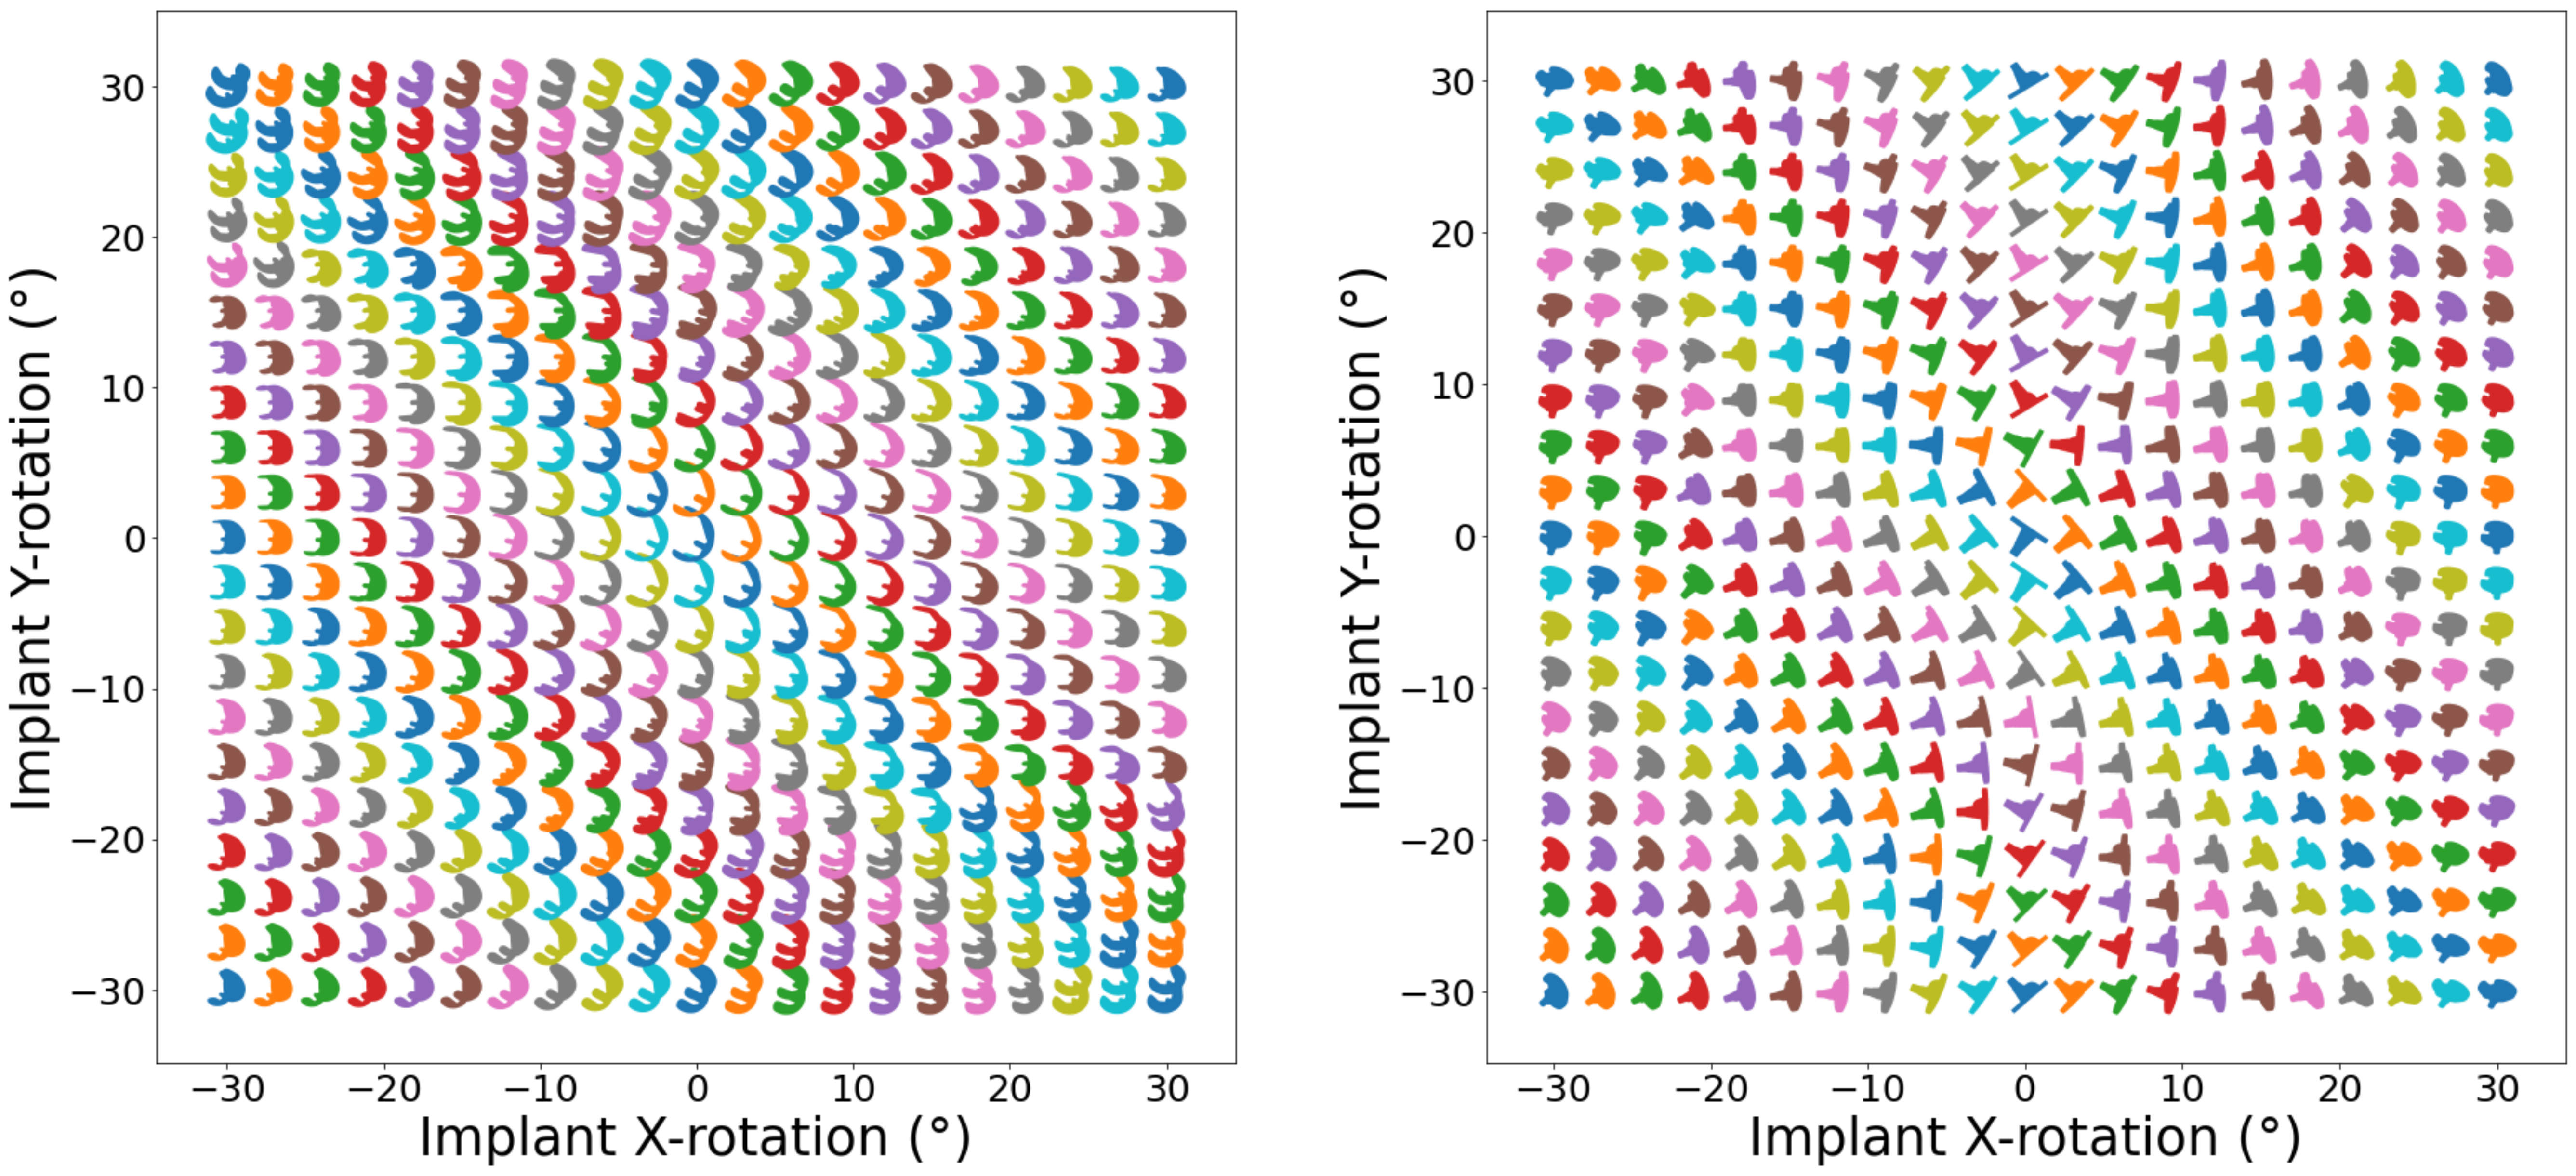
\includegraphics[width = \linewidth]{figs/jtml-paper/fig4-shape-libraries.png}
    \caption{Femoral (left) and tibial (right) NFD shape libraries were generated to capture the variation in projection silhouette geometry with out-of-plane rotation \cite{banksAccurateMeasurementThreedimensional1996}. Initial pose estimates were generated by comparing the NFD contour from the x-ray image to the shape library.}
    \label{fig:nfd-lib}
\end{figure*}

\subsection{Pose Refinement}
A modified Dividing Rectangles (DIRECT) algorithm called DIRECT-JTA  \cite{floodAutomatedRegistration3D2018} generated the final pose estimates. This method of Lipschitzian optimization divides the search into three stages, the “trunk,” “branch,” and “leaf.” Each of the three stages was assigned distinct cost function parameters and search regions. The cost function used a computationally efficient L1-norm between the dilated contour from the segmentation label and the projected implant. Successively decreasing the dilation coefficient allowed the optimization routine to escape local minima, and the leaf branch served to find the optimal out-of-plane translation. Transversely symmetric tibial implants posed problems during registration because two distinct poses produced roughly identical projections \cite{kendallShapeManifoldsProcrustean1984}. Because of this pose ambiguity, the tibial implant was always optimized after the non-symmetric femoral implant. In addition to the dilation metric, the tibial mediolateral translation and varus/valgus rotations relative to the femur were penalized. Final implant poses were transformed into knee joint rotations and translations \cite{groodJointCoordinateSystem1983} and compared to the human-supervised kinematics for the same images using RMS differences for each joint pose parameter. Squared differences between data sets were compared using one-way MANOVA with post-hoc multiple pair-wise comparisons using the Games-Howell test (R v4.2.0 using R Studio, rstatix, and stats).

\subsection{Pose Ambiguities and Registration Blunders}
A blunder was defined as an image frame with the squared sum of rotation differences greater than 5° between autonomous and human-supervised measures. These blunder frames contain errors considerably larger than would be clinically acceptable and warrant further exploration. Blunders were analyzed with respect to the tibial implant’s apparent varus/valgus rotation relative to the viewing ray (Fig. \ref{fig:histo-pdf}). A probability density function and cumulative density function were calculated for the blunder likelihood. Due to the high likelihood of blunders in this region, an ambiguous zone was defined for all apparent tibial varus/valgus-rotation less than 3.6 degrees, which is the mean + 1std of the blunder distribution (Fig. \ref{fig:histo-pdf}). Squared measurement differences between images inside and outside the ambiguous zone were also compared using one-way MANOVA with post-hoc multiple pair-wise comparisons using the Games-Howell test.


\begin{figure*}[hb]
    \centering
    \includegraphics[width = \linewidth]{figs/jtml-paper/fig5-histo.png}
    \caption{The histogram (left) shows the correctly registered frames (Hits, blue) and incorrectly registered frames  (Blunders, orange) plotted as a function of the apparent tibial varus/valgus angle relative to the viewing raw. The probability plot (right) shows the distribution of blunders (solid orange) and the cumulative probability of blunders (dotted orange). The Ambiguous Zone is defined as apparent tibial varus/valgus rotations less than the mean + one standard deviation of the blunder probability distribution, capturing approximately 85 \% of the blunders.}
    \label{fig:histo-pdf}
\end{figure*}


\section{Results}
CNN segmentation of standard test set images produced Jaccard indices of 0.936 for the femoral and 0.883 for the tibial components. CNN segmentation performance on the completely naïve test set was lower, 0.715 and 0.753, respectively.

The initial pose estimates were within the range of convergence for the DIRECT-JTA optimizer and offered a robust initialization for optimization (Table 1). The RMS differences for initial pose estimates on ground-truth images were smaller (better) than for CNN-segmented images, but the differences were mostly within a few millimeters or degrees. Due to poor sensitivity for measuring out-of-plane translation with monocular vision, the mediolateral translation had the largest RMS differences for both image types.



\begin{figure*}[ht]
    \centering
    \includegraphics[width = 0.85\textwidth]{figs/jtml-paper/tab1-nfd-performance.png}
\end{figure*}

RMS differences between DIRECT-JTA optimized kinematics and human-supervised kinematics were sub-millimeters for all in-plane translations (Table II). Mediolateral translations and out-of-plane rotation differences were smaller when the pose of the tibia was outside the ambiguous zone. The RMS differences for the completely naïve test set were within 0.5 mm or 0.5 deg compared to the standard test set, indicating similar performance on the entirely novel dataset.

\begin{figure*}[hb]
    \centering
    \includegraphics[width = 0.93\textwidth]{figs/jtml-paper/tab2-directjta-rms-diff.png}
    \label{tab:direct-rms}
\end{figure*}

There was one femoral blunder and 43 tibial blunders out of 392 test images. Using the definition of the ambiguous zone as apparent tibial varus/valgus rotation less than 3.6 deg, 11\% of images have a tibial blunder within this zone, compared to 3.2\% outside. Sixty-six percent of tibial blunders were due to symmetry ambiguities (Fig \ref{fig:sym-trap}). 


\begin{figure}[!h]
    \centering
    \includegraphics[width = \linewidth]{figs/jtml-paper/fig6-symtrap.png}
    \caption{The figure shows the same radiographic image with two registered tibial implant poses: (a) shows a correctly registered tibial implant, while (b) shows an implant caught in a local cost function minimum corresponding to a nearly symmetric pose.}
    \label{fig:sym-trap}
\end{figure}

One-hundred thirteen image pairs from an RSA study of TKA were used to independently assess the accuracy of the autonomous kinematics measurement for single-plane lateral TKA images. RMS errors were 0.8mm for AP translation, 0.5mm for SI translation, 2.6mm for ML translation, 1.0° for flexion-extension, 1.2° for abduction-adduction, and 1.7° for internal-external rotation. At a different institution, 45 single-plane radiographic images were acquired with an instrumented sawbones phantom that was independently tracked using motion capture. Comparing the motion capture and autonomously measured radiographic kinematics, the RMS errors were 0.72mm for AP translation, 0.31mm for SI translation, 1.82mm for ML translation, 0.56° for flexion-extension, 0.63° for abduction-adduction, and 0.84° for internal-external rotation.

\section{Discussion}
Dynamic radiographic measurement of 3D TKA kinematics has provided important information for implant design and surgical technique for over 30 years. Many surgeons have expressed an interest in utilizing this type of measurement in their clinical practices; however, current methods are impractical. We developed a completely autonomous TKA kinematics measurement pipeline that can potentially provide a practical method for clinical implementation. This study sought to answer three questions, (1) How well does a neural network segment TKA implants from fluoroscopic and flat-panel images? (2) How well can an NFD shape library estimate the pose of a TKA implant given a CNN-segmented image? And (3) How well does a Lipschitzian optimization routine replicate human-supervised kinematics for TKA implants given an approximate initial guess? 

CNN image segmentation of TKA implants worked well, with Jaccard indices greater than 0.88 for the standard test set, and greater than 0.71 for the naïve test set. Segmentation performance for the standard test set outperformed published examples by 0.05-0.1 Jaccard points \cite{zhouUNetNestedUNet2018,rodriguesDeepSegmentationLeverages2019}, with the naïve test set on par with other segmentation examples. The most notable decrease in segmentation performance occurred along the perimeter of the segmented pixel region, especially in areas where implant projections occluded each other. These imperfectly segmented perimeter regions likely affect the initial pose estimate and the DIRECT-JTA optimization solution since both methods rely heavily on the segmented implant boundary. Further improvements can be made for the perimeter segmentation results by introducing intelligent augmentations during training using generative models \cite{hatayaFasterAutoAugmentLearning2019} and performing neural network bolstered contour improvement strategies \cite{yuanSegFixModelAgnosticBoundary2020}. 

Our initial pose estimates were satisfactory as an initialization for the DIRECT-JTA optimization, falling within the convergence region of ±30° \cite{floodAutomatedRegistration3D2018}. However, the performance for the ground-truth projections was not as good as the cited method \cite{banksAccurateMeasurementThreedimensional1996}, which achieved errors of less than 1mm for in-plane translation and 2° for rotation. The cited method utilized an additional refinement step for the NFD estimation, interpolating the apparent out-of-plane angles between nearest shapes in the library. This extra step was not done because only approximate initial pose estimates were needed. In addition, the current study incorporated a vastly larger set of implant shapes (36 vs. 2) and image quality and calibration variations. Distinct implant shapes manifest unique normalization maps, where there can be discontinuities or jumps in normalization angles which affect the best-fitting library entry (Fig. \ref{fig:nfd-lib}) \cite{wallaceAnalysisThreedimensionalMovement1980,wallaceEfficientThreedimensionalAircraft1980}. These details are easily upgraded with additional code using previously reported methods but were not pursued because the initial pose results were well within the DIRECT-JTA convergence region. The initial pose estimates for the CNN-segmented images were not as good as for the ground-truth projections. This follows directly from the fact that the perimeter of the segmented implants was not as accurately rendered, leading to poorer results with the edge-based NFD method. Finally, the out-of-plane translation estimates were relatively poor for both ground-truth projects and CNN-segmented images. This translation estimate is extremely sensitive to model projection and edge detection details and can be adjusted for better results if required. 

RMS differences between human-supervised and DIRECT-JTA optimized kinematics demonstrate the two methods provide similar results. In-plane translation differences of less than 0.8mm and out-of-plane less than 1.8 mm, indicate good consistency in determining the relative locations of TKA implants. Rotation differences of 4° or less for frames within the ambiguous zone, and less than 1.7° for frames outside the ambiguous zone, indicate joint rotation measures with sufficient resolution to be clinically useful. We observed two important characteristics in the measurement comparisons that will affect future implementations and use. First, we identified an ambiguous zone of apparent tibial rotations wherein there is a higher incidence of registration errors. These errors resulted in significant differences in measurement performance for the out-of-plane translations and rotations. This phenomenon, resulting from the nearly symmetric nature of most tibial implants \cite{lavalleeRecoveringPositionOrientation1995,zuffiModelbasedMethodReconstruction1999,banksAccurateMeasurementThreedimensional1996,mahfouzRobustMethodRegistration2003,floodAutomatedRegistration3D2018} prompts either practical modification to imaging protocols to bias the tibial view outside the ambiguous zone or modifications of the model-image registration code to enforce smooth kinematic continuity across image frames and/or to impose joint penetration/separation penalties \cite{muJointTrackOpenSourceEasily2007}. Second, we observed similar measurement performance for the standard and naïve test sets, which differed only in the superior/inferior joint translation. This suggests that the autonomous kinematic processing pipeline can provide reliable measures for implants and imaging systems that were not part of the training set, which will be important for application in novel clinical environments.

Two independent research teams utilized our software to evaluate the accuracy of our autonomous measurement pipeline compared to their reference standard methods using implants and image detectors that were not part of our training sets. In both cases, the accuracy results were comparable to results reported for contemporary human-supervised single-plane model-image registration methods for TKA kinematics \cite{banksAccurateMeasurementThreedimensional1996,floodAutomatedRegistration3D2018, banksVivoKinematicsCruciateretaining1997,banks2003HapPaul2004, komistekVivoFluoroscopicAnalysis2003}. Interestingly, the independent accuracy results appeared superior to our assessment of differences between autonomous and human-supervised measures of TKA kinematics. In both cases, the independent centers used high-resolution flat-panel detectors that provided better spatial resolution and grayscale contrast than most of the imaging systems included in our datasets. With images of similar quality, it is reasonable to expect similar measurement accuracy.  

This work has several limitations. First, the image data sets resulted from previous studies in our labs, so there was no prospective design of which implant systems and image detectors should be included for a pipeline that generalizes well to other implants and detectors. Nevertheless, the naïve data set and the independent assessments, all involving implants and detectors not used for training, performed well and suggest that the method can usefully generalize to measurements of traditionally configured TKA implants. Future work is required to evaluate measurement performance with partial knee arthroplasty or revision implants. Second, many methodologic and configuration options and alternatives remain to be explored, and the current pipeline implementation should not be considered optimal. How best to disambiguate tibial poses and determine the most effective and robust optimization cost functions are areas of current effort.

We present an autonomous pipeline for measuring 3D TKA kinematics from single-plane radiographic images. Measurement reproducibility and accuracy are comparable to contemporary human-supervised methods. We believe capabilities like this will soon make it practical to perform dynamic TKA kinematic analysis in a clinical workflow, where these measures can help surgeons objectively determine the best course of treatment for their patients.

%%% Local Variables:
%%% mode: latex
%%% TeX-master: "../../Andrew_Jensen_Dissertation"
%%% End:

\chapter{Aim 2: Correcting Symmetric Implant Ambiguity in Measuring Total Knee Arthroplasty Kinematics from Single-Plane Fluoroscopy}

\section{Abstract}
Recent advancements in computer vision and machine learning enable autonomous measurement of total knee arthroplasty kinematics through single-plane fluoroscopy.
However, symmetric implants present challenges in optimization routines, causing 'symmetry traps' and ambiguous poses.
Achieving clinically robust kinematics measurement requires addressing this issue. We devised an algorithm that converts a 'true' pose to its corresponding 'symmetry trap' orientation.
From a dataset of nearly 13,000 human supervised kinematics, this algorithm constructs an augmented dataset of 'true' and 'symmetry trap' kinematics, used to train eight classification machine learning algorithms.
The outputs from the highest-performing algorithm classify kinematics sequences as 'obviously true' or 'potentially ambiguous.'
We construct a spline through 'obviously true' poses, and 'ambiguous' poses are compared to the spline to determine correct orientation.
The machine learning algorithms achieved 88-94\% accuracy on our internal test set and 91-93\% on our external test set.
Applying our spline algorithm to kinematics sequences yielded 91.1\% accuracy, 94\% specificity, but 67\% sensitivity.
The accuracy of standard ML algorithms for implants within 5 degrees of a pure-lateral view was 71\%, rising to 88\% beyond 5 degrees.
This pioneering study systematizes addressing model-image registration issues with symmetric tibial implants.
High accuracy suggests potential use of ML algorithms to mitigate shape-ambiguity errors in pose measurements from single-plane fluoroscopy.
Our results also suggest an imaging protocol for measuring kinematics that favors more oblique viewing angles, which could further disambiguate ‘true’ and ‘symmetry trap’ poses.


\section{Introduction}
Measuring total knee arthroplasty (TKA) kinematics from fluoroscopic images has been an important contributor to knee implant design, post-operative assessment, and predictive modeling for wear and failure patterns for nearly 30 years \cite{banksRationaleResultsFixedBearing2019,banks2003HapPaul2004,freglyComputationalWearPrediction2005}.
However, the application of this technology has been limited to research use by the challenges of performing these measurements quickly and reliably, as they often require expensive equipment and time-consuming processes \cite{banksAccurateMeasurementThreedimensional1996,lafortuneThreedimensionalKinematicsHuman1992,zuffiModelbasedMethodReconstruction1999,mahfouzRobustMethodRegistration2003}.
Recent advancements in computer vision and machine learning have opened up the possibility of using a single fluoro-camera for fully autonomous TKA kinematic measurement\cite{brobergValidationMachineLearning2023,jensenJointTrackMachine2023}, making it more accessible and cost-effective for hospitals and clinics.
Nonetheless, this approach faces inherent limitations in accurately resolving orientation and location information using only one fluoro-camera view \cite{banksAccurateMeasurementThreedimensional1996,floodAutomatedRegistration3D2018,mahfouzRobustMethodRegistration2003,yamazakiImprovementDepthPosition2004,zuffiModelbasedMethodReconstruction1999}.

One of the key issues researchers encounter when dealing with imaging from a single camera arises from symmetric implant geometries.
Under a weak perspective/nearly orthographic projection paradigm \cite{szeliskiComputerVisionAlgorithms2022}, symmetric implants have distinct 3D orientations that produce nearly indistinguishable 2-dimensional projective geometry (\cref{fig:symmetry-trap-quadrants}).
Due to the model-image registration process relying on the information present in the 2D fluoroscopic image, this causes multiple local minima for many optimization algorithms.
Human-supervised kinematics measurements for TKA with symmetric tibial implants frequently rely on the relative location of the fibula in the fluoroscopic image to disambiguate the pose.
Unfortunately, fully autonomous solutions can’t utilize this reference point, causing difficulty in algorithmic implementation.

\begin{figure}[h!]
  \centering
  \includegraphics[width=0.78\textwidth]{./figures/raster/sym-trap-quadrants.png}
  \caption{Two examples of symmetry pose dyads with the correct (left) and symmetry trap (right) kinematics. For some orientations, the symmetry trap is obviously incorrect (top), and for others, it is more ambiguous (bottom).}
  \label{fig:symmetry-trap-quadrants}
\end{figure}


In this paper, we utilize 12,592 images from seven studies that utilized human-supervised TKA kinematics \cite{jennyREGISTRATIONKNEEKINEMATICS2015,kefalaAssessmentKneeKinematics2017,okamotoVivoKneeKinematics2011,palm-vlasakMinimalVariationTop2022,scottCanTotalKnee2016,watanabeKneeKinematicsAnterior2013,watanabeInvivoKinematicsHighflex2016} to explore the potential of a novel method to classify and correct 'symmetry trap' poses in single-plane TKA kinematic measurements.
The goal is to improve the accuracy and resolution of single-plane TKA measurements and enable more accessible and reliable kinematic data for orthopaedic applications.

This research paper will answer two key questions:  (1) How effectively can machine learning methods distinguish between 'true' and 'symmetry trap' poses in cases involving symmetric implants? (2) How well can we systematically correct 'symmetry traps' arising in kinematics sequences obtained from fluoroscopic images?

\section{Methods}
\subsection{Study Design and Sample}
In this paper, we are addressing the issue of ‘symmetry traps’ in TKA kinematics measurements from single-plane fluoroscopy.
In order to do so, we take a data-driven approach.
We start with a collection of human-supervised 'true' kinematic measurements, then determine the respective 'symmetry trap' orientation using a novel algorithm.
Using this collection of both ‘true’ and ‘symmetric’ poses, we train eight different machine learning classifiers and evaluate their performance on both an internal and external test set. We then take the highest performing classifier and use it to establish an algorithm that takes as input a contiguous sequence of kinematics measurements, and imposes continuity constraints to fix 'symmetry traps' in real-world data.
We report the performance of our cubic spline correction algorithm on a dataset of autonomously measured kinematics \cite{jensenJointTrackMachine2023}.
All programs were written in Python 3.10.

The dataset used for development of the methodology comprises seven total studies \cite{jennyREGISTRATIONKNEEKINEMATICS2015,kefalaAssessmentKneeKinematics2017,okamotoVivoKneeKinematics2011,palm-vlasakMinimalVariationTop2022,scottCanTotalKnee2016,watanabeKneeKinematicsAnterior2013,watanabeInvivoKinematicsHighflex2016} comprising 12,592 frames of radiographic data.
We completely withheld data from one study \cite{okamotoVivoKneeKinematics2011} during training to use later as an external test set.

\subsection{Determining Symmetric Orientations}
First, 'symmetry trap' poses were identified from 'true' poses through a novel algorithm devised to “flip” any given pose into its symmetric counterpart (\cref{fig:sym-flipper-alg}). The algorithm proceeds as follows:

\begin{enumerate}
  \item Determine the viewing ray from the object origin to the camera origin. Denote this as $\vec{v}$, where $||\vec{v}|| = 1$.
  \item Determine the symmetric axis of the object, $\vec{s}$, where $||\vec{s}|| = 1$. This symmetric axis is equivalent to the normal vector of the ``mirror plane'' of symmetry for the object.
  \item Determine the axis and angle of rotation between $\vec{s}$ and $\vec{v}$ and construct the equivalent rotation matrix.
        \begin{enumerate}
          \item The axis is the cross product, $\vec{m} = \vec{v} \times \vec{s}$.
          \item The angle is the normalized dot product, $\psi = 2 \times \cos^{-1}\dfrac{\vec{v} \cdot \vec{s}}{||\vec{v}||||\vec{s}||}$
        \end{enumerate}
  \item Apply body-centered rotation to the symmetric obhject about $\vec{m}$ by $\psi$.
\end{enumerate}

For each projective geometry, there exist exactly two poses (i.e., a dyad) that produce it, thus applying this algorithm twice will return the original pose.

\begin{figure}[h!]
  \centering
  \includegraphics[width=0.8\linewidth]{./figures/raster/symmetry_flipper.png}
  \caption{A visualization of the ``symmetry flipper'' algorithm that converts 3D orientations into their symmetric counterpart.}
  \label{fig:sym-flipper-alg}
\end{figure}

\subsection{Constructing Dataset}
We collected data from seven studies utilizing human supervised total knee arthroplasty kinematics, totaling approximately 12,592 individual frames.
Anatomic tibiofemoral kinematics were stored as 'true' poses.
The proposed algorithm was then applied to each frame's tibial implant, generating corresponding “symmetric” poses, for a total of 25,184 samples (\cref{fig:sym-trap-dataset}).
Solid angle distances ($\psi$) obtained from the symmetry flipper algorithm were also stored, and the dataset was stratified based on the solid-angle value and split into 67\% training and 33\% testing sets for unbiased evaluation.
Data from one study \cite{okamotoVivoKneeKinematics2011} was completely withheld from training to be used as an external test set.

Thus, for each sample, the input was $\{\theta_{Int/Ext}, \theta_{Flx/Ext}, \theta_{Var/Val}, \psi\}$ with $\theta_{Int/Ext}, \theta_{Flx/Ext}, \theta_{Var/Val}$ representing anatomic internal/external rotation, flexion/extension, and varus/valgus respectively. The target was either `true' or `symmetry trap'.

\begin{figure}[h!]
  \centering
  \includegraphics[width=0.85\textwidth]{./figures/raster/symmetry-trap-dataset.png}
  \caption{A 3D scatter plot of our training data with `true' poses in orange and `symmetry trap' poses in blue. Of note, there are distinct regions of exclusively `symmetry trap' poses, while the region of predominately `true' poises (orange cylinder along Flexion/Extension axis) also has many `symmetry trap' poses.}
  \label{fig:sym-trap-dataset}
\end{figure}
\subsection{Classification Algorithms}
In this study, we implemented a selection of classification algorithms (Table 1) from Scikit-learn \cite{scikit-learn} to distinguish between 'true' and 'symmetry trap' poses.
The chosen algorithms were K-Nearest-Neighbors (KNN) \cite{fixDiscriminatoryAnalysisNanparametric1951},
Support Vector Machines (SVM) \cite{cortesSupportvectorNetworks1995}, AdaBoost \cite{friedmanGreedyFunctionApproximation2001},
Histogram Gradient Boosting \cite{freundDecisionTheoreticGeneralizationOnLine1997},
Bagging Meta-Estimator \cite{breimanBaggingPredictors1996},
Stacked Generalization \cite{smythLinearlyCombiningDensity1999,wolpertStackedGeneralization1992},
and (majority) Voting Classifier.
The hyperparameters for each method were tuned using stratified 5-fold cross validation using grid-search to test all possible combinations.
Stacked generalization and the voting classifier used the tuned hyperparameters from each of the other estimators in their predictions.
We recorded sensitivity \cite{yerushalmyStatisticalProblemsAssessing1947}, specificity \cite{yerushalmyStatisticalProblemsAssessing1947}, accuracy \cite{internationalorganizationforstandardizationAccuracyTruenessPrecision2023},
and the F1 score \cite{tahaMetricsEvaluating3D2015} for each algorithm on our test set.
We also report these metrics of the highest performing individual classifier on stratified partitions of the test set to determine relative performance for different $\psi$ values.


\subsection{Fixing Incorrect Symmetry Trap Poses}
The primary objective of this study is to accurately measure the kinematics of all frames in a TKA kinematics sequence and to robustly fix incorrect symmetry trap poses.
However, due to the inability to know a-priori which poses are `true' and in a `symmetry trap', we must employ a separate procedure for systematically correcting individual frames.
Thus, for every kinematics sequence we employ the following procedure:

\begin{enumerate}
  \item Determining Ambiguous and Non-ambiguous Poses for each frame
        \begin{enumerate}
          \item For each frame, we generate the `symmetric' pose corresponding to the input pose.
          \item We run both the input and its symmetric pose through the highest performing classification algorithm.
          \item If the input pose and its symmetric pose are differently labeled by the classifier (i.e., one is labeled 'true', and the other 'symmetry trap'), take the pose labeled 'true' as the actual pose.
          \item If both poses return the same label (i.e., both 'true' or both 'symmetry trap'), label the pose as “ambiguous” and move to step 2.
          \item If no poses were labeled “ambiguous”, the procedure is finished.
        \end{enumerate}
  \item Constuction of 3-Dimensional cubic b-spline of the movement
        \begin{enumerate}
          \item A spline is individually fit through the flexion/extension, internal/external rotation, and adduction/abduction angles for all frames that were {\bf not} labeled ambiguous.
        \end{enumerate}
  \item Correcting Ambiguous Poses
        \begin{enumerate}
          \item We sample the cubic spline at frame locations of ambiguous poses.
          \item We compare the solid-angle difference between the input and symmetric pose to the pose at the sampled spline location.
          \item Whichever pose is closer to the spline, we take this as the `true' pose.
        \end{enumerate}
\end{enumerate}

To evaluate this procedure, we used a dataset of kinematics generated from a fully autonomous method \cite{jensenJointTrackMachine2023} to emulate the real-world use case of this algorithm as a post-processing operation.
This test set has robustly quantified the presence of `symmetry traps', and so allows us to report sensitivity, specificity, accuracy, and the F1 measure of its ability to correct symmetry traps in a clinical setting.

\section{Results}
\subsection{Machine Learning Classification Performance}
Classification accuracy ranged from 87.8\% to 94.0\%, sensitivity ranged from 92.9\% to 94.7\%, and specificity ranged from 83.5\% to 93.6\% for all eight methods evaluated (Table 1).
Stacked generalization and the voting classifier tended to outperform the other classifiers, as they both incorporated a combination of the other models in their decision-making.
For the external test set (Table 1), the Support Vector Machine with Radial Basis Function kernel had the highest accuracy and F1 score, at 94\% and 0.94 respectively.
Stacked generalization performed slightly worse in the external test set.
Overall, the performance in the external test set was comparable to the performance on the internel test set, with some classifiers seeing decreased performance (K-Nearest-Neighbors, Stacked Generalization), and others seeing slightly increased performance (Support Vector Machines, AdaBoost, Voting Classifer).

\begin{figure}
  \centering
  \includegraphics*[width=0.95\linewidth]{./figures/raster/sym-trap-ML-table.png}
\end{figure}
\begin{figure}
  \centering
  \includegraphics*[width=0.95\linewidth]{./figures/raster/stratified-psi-ML-table.png}
\end{figure}

\subsection{Stratified $\psi$ Test Set Performance}
As the value of $\psi$ increases, the performance of stacked generalization classification increases (Table 2).
At values closer to a pure-lateral view (~0), accuracy is roughly 71\%, and once the implants exceed 5 off-lateral, accuracy increases to above 88\%. See Appendix A for visualization of different test sets.

\subsection{Symmetry Trap Correction Performance}
When applying the procedure to correct symmetry traps, we achieve an accuracy of 91.1\%, a sensitivity of 67.4\% and a specificity of 94\% on an external test set.
The average “distance to symmetric pose” ($\psi$) was  for the frames correctly classified, and  for the frames incorrectly classified.
For our initial internal test set, the distance to the symmetric pose was  for frames correctly classified, and  for incorrectly classified frames.
From this, we can see that the incorrect frames are much closer to a true lateral single-plane image, meaning the difference between the symmetric dyad of poses is smaller.

\section{Discussion}
Orthopaedic surgeons would value a practical method to quantify TKA kinematics clinically for post-operative assessment or exploration of unsatisfactory outcomes \cite{banksWhatPostoperativeOutcome2017}.
To date, research methods for quantifying TKA kinematics from single-plane radiographic images have been too time-consuming for clinical use, but the application of machine learning methods has been rapidly improving their convenience \cite{jensenJointTrackMachine2023}.
A critical step in making this technology ready for clinical use is to address the pose ambiguity issue that arises from single-camera views of symmetric tibial implant components in a time-efficient manner.
We found that several machine learning algorithms were able to robustly identify and correct symmetric erroneous poses with greater than 90\% accuracy, making these measurement methods sufficiently autonomous and robust to be considered for clinical use.


We demonstrated that classical machine learning techniques are extremely adept at handling the classification of 'true' and 'symmetry trap' TKA kinematics measurements from single-plane fluoroscopy.
As a first study in this domain, benchmark comparisons with other metrics, datasets, or algorithms are not available.
However, an accuracy level of at least 87\% establishes a useful performance benchmark in terms of clinical applications of these methods and for future research in this field.
As expected, stacked generalization \cite{wolpertStackedGeneralization1992,smythLinearlyCombiningDensity1999}, where “the worst possible performance is the highest of any individual estimator” held true for our internal test set, and outperformed all other algorithms.
Interestingly, the same trend did not hold for our external test set, which contained kinematics from patients, imaging machines, and surgeons that were completely withheld from training.
In our external test set, SVMs with radial basis function kernel seems to outperform the other classifiers.


Our symmetry trap correction procedure has strong performance in the accuracy ($>91\%$) and specificity ($>94\%$).
We note decreased sensitivity related to decreasing values of our  term, consistent with intuition: when two possible poses are closer together, they are harder to disambiguate.
When performance is measured based on $\psi$ values greater than 5 or 10 degrees, we see that our symmetry trap correction algorithm boasts performance similar to that of the stacked generalization estimator (Table 2).
Previous work has also shown an increase in the prevalence of symmetry traps in low- poses \cite{jensenJointTrackMachine2023}.
We also note that in real-world data, we have imbalanced class representation because most symmetry traps are caught in the initial kinematics measurement, leaving only the most difficult cases for this algorithm to correct.
These reasons both culminate with an expected decreased sensitivity when trying to correct symmetry trap poses.
Future work might be able to address this problem using time-series machine learning algorithms like recurrent neural networks \cite{hochreiterLongShortTermMemory1997} and transformers \cite{vaswaniAttentionAllYou2017} to isolate specific frames that have fallen into symmetry traps based on local and global relationships with other kinematics in that particular sequence.
Additionally, 3D geometries could be used to impose penetration and separation penalties that are further used to refine ambiguous poses.


The performance of autonomous measurements of single-plane fluoroscopy kinematics measurements already achieve clinically acceptable levels of error.
Despite this, measurement errors still occur and roughly 67\% of frames that are incorrectly optimized fall into symmetry traps \cite{jensenJointTrackMachine2023,brobergValidationMachineLearning2023}.
With the techniques proposed in this work, we can drastically improve the overall performance of autonomous single-plane TKA kinematics measurements and remove the largest source of inaccuracy.


Stratifying measurement performance by  (Table 3), it is clear that the joint viewing perspective is a dominant contributor to pose ambiguities.
This suggests a modification to imaging protocols for measuring TKA kinematics to minimize the number of frames that fall into the “ambiguous zone”.
Instead of “pure lateral” imaging that attempts to perfectly center the knee in the image frame, we suggest positioning the center of the knee 1-2 inches away from the center of projection, and to rotate the plane of the observed leg by 5 degrees from parallel with the image detector.
These small adjustments to the imager/patient alignment would cause all kinematics to have >5, which improves classification accuracy by at least 20\%. Similar imaging protocol improvements have been proposed for bi-plane RSA \cite{niesenReorientingTibialBaseplate2020}.
This study has some limitations. In this study, we use human-supervised kinematics from single-plane images, where there is always the possibility that the human operator fell into error when distinguishing between 'true' and 'symmetry trap' poses in a sequence of images. This can occur due to a myriad of factors, including low image quality and near-lateral imaging angles. To mitigate this, validated ground truth kinematics are necessary to create a robust algorithm without any errors in the training data.


The dataset constructed in this study assumes that the femoral implant has been properly registered with correct kinematics.
Often, this is not an issue because most femoral implants are asymmetric, and have an extremely low likelihood of falling into their own 'symmetry traps' \cite{jensenJointTrackMachine2023}.
However, improper registration of both a symmetric tibial implant and symmetric femoral implant would decrease the feasibility of the proposed procedure.


This study presents a novel method of overcoming one of the most pernicious issues facing researchers measuring TKA kinematics from single-plane fluoroscopy.
Our algorithm combines 3 elements (1) calculating 'symmetry trap' poses from 'true' poses, (2) classical machine learning algorithms to classify a single pose as 'true' or 'symmetry trap' and (3) a procedure that applies those machine learning outputs to a contiguous sequence of kinematics to construct a spline and correct symmetry traps in real-world data.
Further, our results suggest slight alterations to imaging angles could reduce errors due to ambiguous poses resulting from symmetrical tibial implants.
We believe that this method, along with recent advancements in autonomous kinematics measurements, will soon make it practical to perform dynamic TKA kinematics measurements in a clinical setting without the inherent limitations of single-plane radiographic imaging.

\section{Conclusion}
Our three-stage approach to correcting 'symmetry traps' that arise from symmetric tibial implants when performing kinematics measurements on single-plane imaging provides a groundbreaking solution to a problem facing researchers in the field for nearly three decades.
Further, the “symmetric flipper” algorithm provides a strong foundational approach for any symmetric object in a weak-perspective paradigm and can drastically reduce the complexity of many optimization algorithms by reducing the search space.
Because this algorithm is model-agnostic, it could be used in many applications where orientation ambiguities arise.
This approach further refines the ability for a fully autonomous kinematics measurement platform, bringing it one step closer to being a clinically viable technology, where these measures can help surgeons objectively determine the best course of treatment for their patients.



%%% Local Variables:
%%% mode: latex
%%% TeX-master: "../../Jensen-Lit-Review"
%%% End:

\chapter{Musings on Latent Kinematics Space and Synthetic Biomechanics Data}

In order to make autonomously measuring joint kinematics a clinically viable tool, the movements and motions being measured must be standardized.
Similar efforts have been put into standardized post-operative outcome metrics like the Knee Society Score (KSS)\cite{insallRationaleKneeSociety1989}, Knee Injury and Osteoarthritis Outcome Score (KOOS) \cite{roosKneeInjuryOsteoarthritis2003}, the Forgotten Joint Score \cite{behrendForgottenJointUltimate2012}, the Western Ontario and McMaster Universities Osteoarthritis Index (WOMAC) \cite{bellamy1988validation}, among others.
Standardizing these metrics enables reliable and objective comparisons across different groups, implants, and surgical techniques.
This same need for standardized metrics exists when quantifying joint kinematics for research and clinical purposes.
Unfortunately, no such standardization exists for quantifying joint kinematics.
While most groups perform similar activities of daily living (Some form of walking, stair rise, chair rise, kneel, lunge, and squat), variations in how these activities are executed hinder direct comparison accuracy.

Thus, this chapter describes a data-driven approach toward being able to select the highest yield activities to be included in a clinical kinematics examination.
To render the autonomous measurement of joint kinematics a viable clinical tool, the time to collect the data must not be excessive, and so a brief and succinct set of activities is preferred.
From these constraints, the first approach stems from the thought, ``All kinematics data is coming from the same patient. Are there underlying characteristics from one activity that translate to all activities?''
An example might arise: ``Can we predict the patient's stair rise kinematics from their walking kinematics?''
The motivating intuition behind these ideas is that they all come from the same patient, and are being driven by the same underlying musculature.
The following chapter will detail the beginning of an experimental procedure, and why the data was insufficient for answering the above questions.
However, another question arises: ``Given the statistical parameters surrounding a ``good outcome'' or ``bad outcome'', might we be able to generated synthetic patient data to overcome the lack of real-world kinematics data?''
This question is particularly relevant in the context of 'big data' and its growing impact.
Many modern algorithms leverage an enormous amount of data, often more than traditional methods of quantified biomechanics are able to generate.
Additionally, HIPAA requirements make it incredibly difficult to share data, slowing down the rapid progress in curated algorithms for biomechanics data that we see with open datasets like ImageNet \cite{russakovskyImageNetLargeScale2015}.

The following chapter will contain some thoughts on solving these problems.

\section{Latent Kinematics Space and Reducing the Number of Movements Required for a Full Kinematics Evaluation}
\label{sec:latent-kinematics-space}
The concept of latent space in kinematics is analogous to the latent spaces found in other domains, such as natural language processing (NLP).
In NLP, latent space refers to the underlying, hidden structure in language data that algorithms attempt to uncover \cite{jurafskySpeechLanguageProcessing2009}.
This is where the power of transformers \cite{vaswaniAttentionAllYou2017} in NLP becomes relevant to our study of kinematics.

In kinematics, each movement pattern can be thought of as a unique ``expression'' of the underlying musculoskeletal system, akin to how sentences are expressions of underlying linguistic rules and meanings in language.
By exploring the latent kinematics space, we aim to reduce the number of movements required for a comprehensive kinematics evaluation without losing the predictive power or statistical significance of the evaluation.
This approach is based on the hypothesis that certain movement patterns contain redundant information, which could be inferred from other, more distinct movements.
For instance, we might predict the kinematics of a ``stair rise'' from the ``walking'' pattern, assuming that the essential biomechanical information is embedded within the walking movement.

Test

%%% Local Variables:
%%% mode: latex
%%% TeX-master: "../../Jensen-Lit-Review"
%%% End:



\section{Toward Generating Synthetic Biomechanics Data}
\label{sec:synthetic-biomechanics-data}
Many of the issues encountered during the ``kinematics translator'' are directly applicable to generating synthetic kinematics data as well.
At the core, the fundamental problem is the same: we want to convert an interpretable latent space into some kinematics measurement that can be used for neural network training for kinematics analysis.
However, this still requires a robust latent space from which we draw from to generate the synthetic data, which runs into exactly the same difficulties as trying to build a kinematics translator.
The lack of standardization of kinematics measurements, as well as consistently reported post-operative outcomes, means that it would be nearly impossible to train a latent space that is both interpretable (e.g. being able to generate a ``healthy'' or ``failing'' kinematics sequence) and robust (i.e. $\xi_{\phi} \pm \delta = \xi$).

One of the main benefits of having a tool to easily, accurately, and autonomously measure kinematics data is that the door will be open to creating standard procedures for these measurements.
The next steps toward utilizing this technology in a clinical setting will be establishing a framework for all clinicians and researchers to use when performing a kinematics evaluation.
With the spread of anonymized health datasets, a kinematics dataset containing thousands of patients all performing the same activities, and each having the same post-operative metrics recorded, would pave the way for quantitative assessment and correlation of kinematics data to outcome.

%%% Local Variables:
%%% mode: latex
%%% TeX-master: "../../Jensen-Lit-Review"
%%% End:





%%% Local Variables:
%%% mode: latex
%%% TeX-master: "../../Andrew_Jensen_Dissertation"
%%% End:

\chapter{This Will Definitely Work on Shoulder Implants, Right?\protect\footnotemark}
\footnotetext{No}

\section{Introduction}
Another common arthroplasty (TSA) procedure is total shoulder replacement, which involves the removal and replacement of the distal end of the glenoid/scapula and the proximal end of the humeral head.
Researchers, implant manufacturers, and surgeons, driven by similar motivations for understanding post-operative Total Knee Arthroplasty (TKA) kinematics, show equal interest in examining post-operative TSA kinematics.
Despite differing from TKA outcomes, a significant portion of TSA patients report dissatisfaction, predominantly attributing it to mechanical limitations or instability.

For the past twenty years, researchers have explored both anatomical and reverse total shoulder arthroplasty kinematics \cite{kijimaVivo3dimensionalAnalysis2015,matsukiVivo3DAnalysis2014,matsukiDynamicVivoGlenohumeral2012,sugiComparingVivoThreedimensional2021,burtonFullyAutomaticTracking2023}, attempting to draw connections between different implants and surgical techniques to postoperative shoulder dynamics and range of motion.
For the same reasons that a reliable, fast, clinically practical, and fully-autonomous kinematics measurement platform would be desirable for clinicians operating on post-operative total knee arthroplasty (\cref{sec:jtml}), it would also be desirable for clinicians working on total shoulder arthroplasty.

Unfortunately, applying the same pipeline to shoulder implants did not work.
This dissertation chapter is divided into three sections.
First, I will discuss the methods and results of applying our existing framework to the problem of measuring TSA implant kinematics, and explain some of the pitfalls.
Second, I will dive into some of the modifications made to the model-image registration cost-function to try and overcome some of the TSA kinematics limitations.
Last, I will discuss a geometric first-principles approach used to dive even deeper into diagnosing the inherent kinematics measurement issues, and propose of methodological recommendations for others wishing to perform these measurements.
This last chapter will be converted into a paper for hopeful publication.

\section{JointTrack Machine Learning on Total Shoulder Arthroplasty Implants}
\subsection{Introduction}
The successful application of Joint Track Machine Learning (JTML) to Total Knee Arthroplasty (TKA) implants suggested potential applicability to other implant types and joints.
This hypothesis was supported by JTML's robust performance across varied TKA implant styles, including posterior stabilized and cruciate retaining designs, and differences in the peg design of the tibial baseplate.
Consequently, we replicated the TKA experimentation framework, applying it to Total Shoulder Arthroplasty (TSA) implant data, to assess whether this success could be mirrored in a different joint context.

\subsection{Methods}
We sourced 823 post-operative reverse TSA (rTSA) images with human-supervised kinematics from Nagoya University, adhering to IRB guidelines.
These images were obtained using single-plane fluoroscopy to measure glenohumeral kinematics in patients performing anonymized movements.
The collected data for each patient included deidentified radiographic images, imaging calibration files, and manufacturer-supplied glenoid and humeral implant surface geometry files.


We employed the same convolutional neural network (CNN) architecture previously used for TKA implants \cite{wangDeepHighResolutionRepresentation2020} (\cref{sec:jtml}) maintaining an 80/20 training/testing split.
A key consideration was the relative scarcity of rTSA images compared to TKA.
To address this, we augmented the training set with non-affine transformations, specifically grid distortion and elastic transform \cite{buslaevAlbumentationsFastFlexible2020}.
While such transformations increased training times in the TKA pipeline, their computational intensity was manageable given the smaller rTSA image dataset, enhancing the network's generalization capability for rTSA image segmentation.

Next, we applied the DIRECT-JTA algorithm from the JTML suite to rTSA images, evaluating our autonomous kinematics measurement platform.
The efficacy of the algorithms will be assessed by comparing the root-mean-square difference between autonomous and human-supervised kinematic measurements on this novel test set.

\subsection{Results}

%%% Local Variables:
%%% mode: latex
%%% TeX-master: "../../Andrew_Jensen_Dissertation"
%%% End:

\section{Improving Model-Image Registration}
\label{sec:new-image-metrics}
\subsection{Introduction}
Due to the relatively poor performance of the standard optimization algorithm (DIRECT \cite{jonesLipschitzianOptimizationLipschitz1993,floodAutomatedRegistration3D2018}) and the cost function ($L_{1}$-distance or Hamming Distance \cite{floodAutomatedRegistration3D2018}), the first step was to determine whether a more robust representation of image similarity might offer a stronger performance (\cref{sec:image-similarity}).
There are a few approaches that were used to determine a more robust image similarity description that might make it easier to find a global minima for this model-image registration problem.

Firstly, we considered enhancing the convexity of the problem.
In the current formulation, the cost is at its maximum error ($\sum I + P$) when there is no overlap between the projection and the CNN, regardless of whether the projection is off by 5 pixels or 500 pixels.
This issue necessitates a more nuanced error gradient.

Secondly, we delved into the psychology of shape.
Since manual registration serves as the benchmark for ground-truth kinematics, understanding human perception of shape differences and overlaps is crucial.

Lastly, consultations with surgeons and engineers experienced in manual kinematics measurements were sought. Their insights into effective procedures and features for accurate registration are invaluable for refining our approach.

There were some constraints when exploring the addition of new cost parameters for Joint Track Machine Learning.
Primarily, no new cost functions could conflict with the established Hamming Distance, meaning all additional metrics must reach their minimum concurrently with the Hamming distance.
Additionally, the algorithm needed to support parallel processing in CUDA without significantly increasing the computational load per image.
Maintaining the current efficiency, where only one error kernel is required per iteration, was crucial to preserve application performance.

\subsection{Improving Error Gradient}
In order to improve the gradient, some notion of ``closeness'' and ``farness'' needs to be established in the image plane, beyond just ``hits'' and ``misses'' that are counted during the Hamming distance.

The general class of functions that satisfy this propery, while also offering consistent minima with the Hamming distance are called \textit{surface distances} \cite{reinkeCommonLimitationsImage2023,reinkeUnderstandingMetricrelatedPitfalls2023}.
A surface distance is exactly the mathematical formulation that captures this notion of ``closeness'' or ``farness'' from one contour to another contour in an image plane.
A sub-distinction of surface distances are \emph{symmetric surface distances}, in which $d(a,b) = d(b,a)$, but this need not be the case for a useful metric.
There are four main recommended metrics for evaluating the surface distance.

The first is the Normalized Surface Distance or Normalized Surface Dice (\Cref{fig:surfDICE}) \cite{nikolovClinicallyApplicableSegmentation2021} .
Unfortunately, surface DICE runs into the same issue as Hamming distance where it is maximized at points of no overlap, but does not make true distinctions between closer and farther estimations.

\begin{figure}[h!]
  \centering
  \includegraphics[width=0.9\textwidth]{~/figures/raster/NSD.png}
  \caption{A graphical representation of the Normalized Surface Distance from \cite{reinkeUnderstandingMetricrelatedPitfalls2023,reinkeCommonLimitationsImage2023}}.
  \label{fig:surfDICE}
\end{figure}

The second is the Mean Average Surface Distance or Mean Surface Distance (\Cref{fig:MASD}) \cite{benesPerformanceEvaluationImage2015}.
This measures the \emph{mean} of the \emph{averages} over all shortest distances from all points on one boundary to any point on another boundary \cite{reinkeCommonLimitationsImage2023,reinkeUnderstandingMetricrelatedPitfalls2023}.
A major pitfall of this method is that calculating the average distance to the estimation would require spawning one sub-kernel per sampled pixel on the target and estimated contour, which would increase the number of computations by multiple orders of magnitude.

\begin{figure}[h!]
  \centering
  \includegraphics[width=0.9\textwidth]{~/figures/raster/MASD.png}
  \caption{A graphical representation of the Mean Average Surface Distance from \cite{reinkeCommonLimitationsImage2023,reinkeUnderstandingMetricrelatedPitfalls2023}}.
  \label{fig:MASD}
\end{figure}

The third is the Average Symmetric Surface Distance (\Cref{fig:ASSD}) \cite{yeghiazaryanFamilyBoundaryOverlap2018}.
This is a symmetric variation of the mean average surface distance, which does not take the mean of the average shortest distances, but rather just the average distance from both contours to the other contour.
This encounters the same issue as the Mean Average Surface Distance, requiring sub-kernels to calculate distances for each sampled point, drastically increasing the required number of computations per iteration.

\begin{figure}[h!]
  \centering
  \includegraphics[width=0.9\textwidth]{~/figures/raster/ASSD.png}
  \caption{A graphical representation of the Average Symmetric Surface Distance from \cite{reinkeUnderstandingMetricrelatedPitfalls2023,reinkeCommonLimitationsImage2023}}.
  \label{fig:ASSD}
\end{figure}

The last is the Hausdorff Distance (\Cref{fig:HD}) \cite{huttenlocherMultiresolutionTechniqueComparing1993,felzenszwalbDistanceTransformsSampled2012,huttenlocherComparingImagesUsing1993}.
The Hausdorff distance is the maximum distance from a point on one boundary to the nearest point on another boundary. Typically the Hausdorf distance for an entire countour is taken as the average of the Hausdorff distances for a series of sampled points on the target contour.
Like the previous two, the Hamming distance requires sub-kernels for every sampled point, and so it is not feasible.


\begin{figure}[h!]
  \centering
  \includegraphics[width=0.9\textwidth]{~/figures/raster/HausdorfDistance.png}
  \caption{A graphical representation of the Hausdorff Distance, taken from \cite{reinkeCommonLimitationsImage2023,reinkeUnderstandingMetricrelatedPitfalls2023}}.
  \label{fig:HD}
\end{figure}

At this point, all recommended distance metrics do not satisfy our criteria for a feasible cost function that introduces an error gradient.
Based on the pitfalls of each of the above, the ability to pre-compute as many values as possible in order to reduce the algorithmic load during optimization seems ideal.
In previous work, 3D distance maps were pre-computed to perform medical model-image registration \cite{lavalleeRecoveringPositionOrientation1995,zuffiModelbasedMethodReconstruction1999}.
And so, a cost function was devised that can utilized pre-computed distance maps to introduce an error gradient, without needing to spawn multiple kernels during each iteration of optimization.

\subsection{Modified Mean Distance Cost Function}
First, rather than looking at an average distance of all points on the target (a process which spawns multiple sub-kernels), we introduce a distance map which encodes the distance to the \emph{closest point} on the target contour.

With an arbitrary image point defined as $p_{xy}$, and the target contour defined as $T$, we can express this distance map as a grid, $\displaystyle DM_{xy}(T) = \min_{t\in T}d(p_{xy},t)$, where $d(p_{xy},t)$ is any distance function that you want to use. In our case, we use the $L_{1}$-distance for efficient computation.

And then, one can express a notion of distance between the projected contour and the target contour by taking the average of the element-wise multiplication between the projection and the pre-calculated distance map (\cref{eq:DMCF}).
This has the major benefit of only needing a single kernel for each iteration (we are only iterating once per projection and performing a multiplication and atomic addition in memory) as well as sharing a minimum with the Hamming distance.
We can see this by noticing that $DM_{x,y}=0$ for points on the target contour, and so, if $Proj_{x,y}$ were perfectly aligned with this contour, our summation would simply be adding zeros.

\begin{equation}
  \label{eq:DMCF}
  J = \dfrac{ \sum_{(x,y) \in \text{Image}} Proj_{x,y}DM_{x,y} }{\sum_{(x,y)\in \text{Image}}Proj_{x,y}}
\end{equation}

Unfortunately, the results of this endeavor do not improve the overall performance of the DIRECT algorithm in finding a global minima for rTSA implants.
The performance is very similar to the poor performance noticed during the Hamming distance.


%%% Local Variables:
%%% mode: latex
%%% TeX-master: "../../Jensen-Lit-Review"
%%% End:

\section{2D Shape Projection Sensitivity Analysis}
\label{sec:shape-sensitivity}
\subsection{Introduction}


The application of Joint Track Machine Learning to reverse Total Shoulder Arthroplasty (rTSA) implants has unfolded a complex scenario.
It highlights the intricate relationship between optimization algorithm performance, specific cost functions, and the inherent shape of the 3D models used for registration.
A particular challenge lies in the intrinsic properties of humeral models, which present unique difficulties in model-image registration.
To address these challenges, a thorough understanding of the relationship between a 3D shape and its projective geometry is crucial.
This understanding is expected to shed light on the stark differences in algorithmic performance between total knee arthroplasty (TKA) and rTSA implants.


Understanding shape and its salient features has been a crucial aspect of computer vision since it was intertwined with psychology and neurology \cite{attneaveInformationalAspectsVisual1954,attneaveQuantitativeStudyShape1956}.
Many intuitively appealing ideas about shape, such as the salience of curvature and vanishing points in projections, required mathematical definition to be effectively incorporated into image processing algorithms.
Invariant Shape Descriptors, which remain consistent across rigid transformations or scaling, are particularly significant \cite{zhangReviewShapeRepresentation2004}.
These descriptors encapsulate the essence of a shape, independent of factors like rotation, scaling, or position in an image.
Normalized Fourier Descriptors are among the most notable examples of invariant shape descriptors that have been used for aircraft recognition \cite{wallaceEfficientThreedimensionalAircraft1980,wallaceAnalysisThreedimensionalMovement1980,richardIdentificationThreeDimensionalObjects1974}, aerial photography classification \cite{linClassificationPartial2D1987}, model-image registration \cite{zossoBiplanar2Dto3DRegistration2008}, and even measuring TKA kinematics from single-plane images \cite{banksAccurateMeasurementThreedimensional1996}.
Hu moments \cite{huVisualPatternRecognition1962}, the Hough Transform \cite{ballardGeneralizingHoughTransform1981}, Shape Context \cite{belongieShapeMatchingObject2002}, Curvature scale space \cite{koenderinkSurfaceShapeCurvature1992}, the Angular Radial Transform \cite{leeNewShapeDescription2012}, and multi-scale Shape Descriptors \cite{al-thelayaInShaDeInvariantShape2021} have all been proposed as robust methods for vectorizing a shape into mathematically comparable elements.

The central inquiry of this chapter is whether a robust binary shape descriptor can elucidate the relative underperformance of model-image registration for rTSA implants compared to TKA implants. This question not only addresses a specific technical challenge but also aims to contribute to the broader understanding of shape analysis in medical imaging.

\subsection{Methods}
\subsubsection{Data Collection}
First, we collected one manufacturer-provided model from each of: rTSA humeral implant, rTSA glenosphere implant, TKA femoral implant, and TKA tibial implant for testing shape sensitivity.
\subsubsection{Image Generation}
The binary silhouette of each implant was rendered using an in-house CUDA camera model (CUDA Version 12.1) \cite{nickollsScalableParallelProgramming2008} to a $1024\times 1024$ image plane.
The focal length of the pinhole camera model was 1000mm and each pixel was 0.3mm.
All CUDA programming was performed on an NVIDIA Quadro P2200 GPU.
\subsection{Invariant Angular Radial Transform}
The invariant angular radial transform descriptor (IARTD) was selected due to its sensitivity in the radial direction \cite{leeNewShapeDescription2012}.
This sensitivity allows us to address minor changes along the contour of our projected shape, which is a desirable property for determining the minor changes in shape with respect to input orientation.

The IARTD is a complex moment calculated by summing orthogonal basis components on the unit polar disk.
Each basis function has an order ($n$) and a repetition ($p$).
Intuitively, the order represents concentric ``rings'' in our polar disk, and the repetition is the number of ``pie slices'' in our unit disk along $\theta$.
To perform these calculations, we normalize our image such that $(0,0)$ is at the center and $(\pm1,\pm1)$ are the four corners.

Each angular radial transform (ART) coefficient is a complex double integral (\cref{eq:F_np}) over the image in polar coordinates, $f(\rho,\theta)$ multiplied by the ART basis function, $V_{np}(\rho,\theta)$ (\cref{eq:V_np}).

\begin{equation}
	\label{eq:F_np}
	F_{np} = \int_{0}^{2\pi}\int_{0}^{1}f(\rho,\theta)V_{np}(\rho,\theta)\rho d\rho d\theta
\end{equation}

\begin{equation}
	\label{eq:V_np}
	V_{np}(\rho,\theta) = A_{p}(\theta)R_{n}(\rho)
\end{equation}

Our radial basis function is comprised of a complex exponential, $A_{p}(\theta)$ (\cref{eq:A_p}), which provides rotational invariance, and a trigonometric transform, $R_{p}(\theta)$ (\cref{eq:R_n}) to provide orthogonality.

\begin{equation}
	\label{eq:A_p}
	A_{p}(\theta) = \dfrac{1}{2\pi}e^{jp\theta}
\end{equation}
\begin{equation}
	\label{eq:R_n}
	R_{n}(\rho) =
	\begin{cases}
		1                   & n=0     \\
		2 \cos (\pi n \rho) & n \ne 0
	\end{cases}
\end{equation}

Lastly, in order to correct for differences in the in-plane rotation, we apply a phase-correction to each ART coefficient (\cref{eq:art_phase_correction}, \cref{eq:fnp_phase_correction}).
\begin{equation}
	\label{eq:art_phase_correction}
	\phi'_{np} = \phi_{np} - \phi_{n,1}
\end{equation}

\begin{equation}
	\label{eq:fnp_phase_correction}
	F_{np}' = F_{np}e^{-jp\phi_{n,1}}
\end{equation}

And the, the final feature vector becomes a the polar decomposition of our coefficient at each order and repetition \cref{eq:iartd}.
We exclude values from the first two repetitions because they contain no valuable information.
To construct the full IARTD feature vector, we used values of $n=\{0, \dots, 3 \}$ and $p=\{0, \dots, 8\}$.

\begin{equation}
	\label{eq:iartd}
	IARTD = \{|F'_{np}|, \phi_{np}'\} \text{ where } n \ge 0, p \ge 2
\end{equation}

\subsubsection{Shape Differences and Sensitivity}
The primary goal of this section is to establish a easily interpretable value that captures the overall change from one shape to another.
For clarity in representation, successive rotations were denoted as subscripts, such that $R_{z}R_{x}R_{y} = R_{z,x,y}$. The application of the IARTD equation to an implant at a specific input orientation $R_{z,x,y}$ was represented as $IARTD(R_{z,x,y})$.
Shape differences were calculated using the central difference equation on the IARTD vector produced from two different orientations.
The grid of sampled orientations had extrema of $\pm 30$ with a step size of $5$ for each of the $x$, $y$, and $z$ axes.
The ``differences'' along each axes were computed by applying a positive and negative rotation ($\pm \delta $) of 1 degree.
And so, for every input $x,y,z$ rotation, there will be three shape differences, one for each $\delta_{x}$, $\delta_{y}$ or $\delta_{z}$ (\cref{eq:shape-derivative}).
For notational brevity, we will condense the full equation down to a single $\Delta S(\delta)$, (representing $\Delta Shape$ for a differential rotation $\delta$).

\begin{equation}
	\label{eq:shape-derivative}
	\Delta S(\delta)_{z,x,y} \equiv \dfrac{ \partial IARTD(R_{z,x,y}) }{\partial \delta} \propto IARTD(R_{z,x,y,+\delta}) - IARTD(R_{z,x,y,-\delta})
\end{equation}

Because each element of the IARTD vector is at a different scale, we must standardize each element in order to ensure accurate assessment of global behavior without analysis being dominated by a single value.
We use z-score to do this, which assumes a normal distribution, but allows for some outliers if they are present.


After z-scaling, we took the Euclidean norm of each $S(\delta)_{z,x,y}$ to capture the total amount of change of that shape for a given differential rotation (\cref{eq:euc_norm}).
Our final step takes advantage of two factors: first, that our in-plane rotations are the first in our Euler sequence ($z$-axis), and second, that this type of rotation does not affect the in-plane shape.
And so, for every $x$ and $y$ input rotation, we average all the values where $x$ and $y$ are held constant as $z$ varies (\cref{eq:z_rot_norm}).
This yields our final values, which we will denote $\mathbb{S}$.
$\mathbb{S}_{x,y}$ will have separate plots for each $x$, $y$, and $z$ differential rotation and for each of the four implants.
These plots will be compared with respect to JTML optimization performance and regions of difficulty for optimization.


\begin{equation}
	\label{eq:euc_norm}
	\|S(\delta)_{z,x,y}\|_{2}
\end{equation}

\begin{equation}
	\label{eq:z_rot_norm}
	\mathbb{S}(\delta)_{x,y} = \dfrac{\sum_{z} \| S(\delta)_{z,x,y} \|_{2}}{N}
\end{equation}

\subsection{Results}

The average value of $\mathbb{S}(\delta_{y})$ for the humeral implant was much lower than all other implant types (\cref{fig:hum_sensitivity_plot}) (\cref{tab:ss-vals}).
This rotation represents the final rotation in our Euler rotation sequence (Z-X-Y) and captures the internal/external rotation of the humeral implant.
The average $\delta_{x}$ value for our humeral implant was the largest among all implants (\cref{tab:ss-vals}).
Additionally, the surface plotted by the humeral shape sensitivity for all $\delta_{x,y,z}$ is much smoother than any of the other plots, demonstrating the relative lack of shape difference for a wide range of input orientations.
Many other plots had regions of relative in-sensitivity, like the glenosphere $\delta_{y}$ sensitivity along the $y=0$ axis (\cref{fig:sca_sensitivity_plot}) and the tibial $\delta_{y}$ sensitivity along the $x=0$ axis (\cref{fig:tib_sensitivity_plot}).
The femoral implant had the highest average sensitivity ($\frac{\mathbb{S}(\delta_{x}) +\mathbb{S}(\delta_{y}) +\mathbb{S}(\delta_{z})  }{3}$) among all implant types .


\begin{table}
	\caption{Average projected-shape sensitivity values for each of the implant models.} \label{tab:ss-vals}
	\begin{tabularx}{\textwidth}{|X|X|X|X|}\hline
		{\bf Implant Type} & Average $\mathbb{S}(\delta_{x})$ & Average  $\mathbb{S}(\delta_{y})$ & Average $\mathbb{S}(\delta_{z})$ \\ \hline
		Humeral            & 8.83                             & 4.82                              & 7.08                             \\\hline
		Glenosphere        & 6.37                             & 6.22                              & 4.86                             \\\hline
		Femoral            & 6.88                             & 8.68                              & 4.93                             \\\hline
		Tibial             & 9.0                              & 5.52                              & 3.72                             \\\hline
	\end{tabularx}
\end{table}


\begin{figure}[h!]
	\centering
	\includegraphics[width=0.3\linewidth]{~/figures/raster/Humeral_dx_sensitivity.png}
	\includegraphics[width=0.3\linewidth]{~/figures/raster/Humeral_dy_sensitivity.png}
	\includegraphics[width=0.3\linewidth]{~/figures/raster/Humeral_dz_sensitivity.png}
	\caption{The $\mathbb{S}$ plot for a humeral implant for $\delta$ rotations along the x, y, and z axis, respectively.}
	\label{fig:hum_sensitivity_plot}
\end{figure}

\begin{figure}[h!]
	\centering
	\includegraphics[width=0.3\linewidth]{~/figures/raster/Glenosphere_dx_sensitivity.png}
	\includegraphics[width=0.3\linewidth]{~/figures/raster/Glenosphere_dy_sensitivity.png}
	\includegraphics[width=0.3\linewidth]{~/figures/raster/Glenosphere_dz_sensitivity.png}
	\caption{The $\mathbb{S}$ plot for a glenosphere implant for $\delta$ rotations along the x, y, and z axis, respectively.}
	\label{fig:sca_sensitivity_plot}
\end{figure}
\begin{figure}[h!]
	\centering
	\includegraphics[width=0.3\linewidth]{~/figures/raster/Femoral_dx_sensitivity.png}
	\includegraphics[width=0.3\linewidth]{~/figures/raster/Femoral_dy_sensitivity.png}
	\includegraphics[width=0.3\linewidth]{~/figures/raster/Femoral_dz_sensitivity.png}
	\caption{The $\mathbb{S}$ plot for a femoral implant for $\delta$ rotations along the x, y, and z axis, respectively.}
	\label{fig:fem_sensitivity_plot}
\end{figure}
\begin{figure}[h!]
	\centering
	\includegraphics[width=0.3\linewidth]{~/figures/raster/Tibial_dx_sensitivity.png}
	\includegraphics[width=0.3\linewidth]{~/figures/raster/Tibial_dy_sensitivity.png}
	\includegraphics[width=0.3\linewidth]{~/figures/raster/Tibial_dz_sensitivity.png}
	\caption{The $\mathbb{S}$ plot for a tibial implant for $\delta$ rotations along the x, y, and z axis, respectively.}
	\label{fig:tib_sensitivity_plot}
\end{figure}


\subsection{Discussion}
The results shown align with many of our intuitive expectations about measuring the sensitivity of projected shape with respect to 3D object orientation, as well as aligned with the regions of difficulty for JTML optimization.
The humeral implant demonstrated an overall smooth and low shape sensitivity, especially for $\delta_{y}$ rotations (\cref{tab:ss-vals}).
This axis is the axis along which the humeral implant is the most cylindrical, which means that we would not expect to see a large change in the shape descriptor with minor $\delta_{y}$ rotations.
Additionally, this is the axis which JTML had the most difficulty with.

We see similar intuitive results in the glenosphere implant, which had the lowest average $\mathbb{S}(\delta)$ value among all implant types.
This bulk of the volume of this implant is the articulation surface, which closely resembles a sphere.
Because the projection of a sphere (a circle) is unchanging with respect to the orientation of a sphere, we would expect that the more closely a shape resembles a sphere, then we should expect a lower overall shape sensitivity.

We see that the shape sensitivity of the tibial implant along the $\delta_{y}$ rotation corroborates our intuition about symmetry traps.
Along the line defined by $x=0$, we see a consistently low shape sensitivity.
This internal/external rotation axis is exactly the axis that caused issues with symmetry traps, wherein 2 distinct 3D orientations produce the same projected shape.
In the context of this discussion, we would say that the $\Delta S = 0$ between those two tibial orientations.

Another aspect of Joint Track Machine Learning that this study informs is the current use of Euler angles in our DIRECT-JTA optimization routine.
Rather than independently varying all angles in a body-centered reference frame, which is insuitable for hyperbox creation, we are presently optimizing over a range of ordered rotations projected via the sequence $R_{z}R_{x}R_{y}$.
As evidenced by the humeral implant's struggles aligning the $y$-axis, this ordered sequence with a symmetric final axis can impede convergence.

Beyond the inherent shape sensitivities, such optimization limitations motivate exploring alternatives to Euler angles.
Performing registration optimization directly on the Special Orthogonal group $SO(3)$ poses an intriguing direction.
$SO(3)$ encapsulates all possible 3D rotations in a mathematically convenient structure (A \emph{Lie Group}, which is both a manifold and a group).
By optimizing on this manifold instead of using specific angle parametrizations, issues with gimbal lock and cascade effects can be avoided.
Optimization over Lie groups is an emerging subfield - establishing robust $SO(3)$-based registration cost functions could significantly improve JTML convergence while relying less on descriptor sensitivity along certain axes.

\subsubsection{Code Examples}


\begin{lstlisting}
  // IARTD.cpp
std::vector<float> calculateIARTD(img_desc* img_desc_gpu,
                                  gpu_cost_function::GPUImage* dev_image) {
    /**
     * This is a function to calculate the Invariant Angular Radial Transform
     Descriptor.
     * See: J.-M. Lee and W.-Y. Kim, A New Shape Description Method Using
     Angular Radial Transform, IEICE Trans. Inf. \& Syst., vol. E95.D, no. 6,
     pp. 1628-1635, 2012, doi: 10.1587/transinf.E95.D.1628.
     * The input is a binary image (either a segmentation or a projected image),
     and the output is the vector containing the descriptor variables.
     */
    const int MAX_P =
        8;  // Setting max values for the number of "rings" and "angles"
    const int MAX_N = 3;
    float phase_n_1[MAX_N + 1];  // Creating array for phase correction term
    // (Eqs 15, 16)
    int H = img_desc_gpu->height();
    int W = img_desc_gpu->width();
    std::vector<float> iartd(2 * (MAX_N + 1) * (MAX_P + 1));

    auto idx = [](int n, int p) -> int {
        return (n * MAX_P + p - 1) * 2;
    };  // Lambda for easy indexing
    for (int n = 0; n <= MAX_N; n++) {
        for (int p = 0; p <= MAX_P; p++) {
            std::complex<float> fnp = img_desc_gpu->art_n_p(n, p, dev_image);
            if (p > 1) {
                iartd[idx(n, p)] = abs(fnp) / (float)(H * W);
                iartd[idx(n, p) + 1] = arg(fnp) / (float)(H * W);

            } else if (p == 1) {
                // But, we want to keep values at p=1 for the normalization
                // procedure
                phase_n_1[n] = arg(fnp);
            }
        }
    }
    // Phase Correction using values from p = 1 (Eq 15, 16)
    for (int n = 0; n <= MAX_N; n++) {
        for (int p = 2; p <= MAX_P; p++) {
            std::complex<float> fnp_prime =
                std::complex<float>(iartd[idx(n, p)], iartd[idx(n, p) + 1]) *
                exp(std::complex<float>(0.0, -p * phase_n_1[n]));
            iartd[idx(n, p)] = abs(fnp_prime);
            iartd[idx(n, p) + 1] -= phase_n_1[n];
        }
    }
    return iartd;
'';
\end{lstlisting}

\begin{lstlisting}
  // IARTD.cu
  // These are the associated CUDA Kernels for IARTD Calculations
__global__ void art_np_kernel(int height, int width, int n, int p,
                              unsigned char* image, float* dev_fnp_re,
                              float* dev_fnp_imag, int left_x, int bottom_y) {
    // thread values
    int thread_x = (blockIdx.x * blockDim.x) + threadIdx.x;
    int thread_y = (blockIdx.y * blockDim.y) + threadIdx.y;

    int x = thread_x + left_x;
    int y = thread_y + bottom_y;

    int orig_loc = x + width * y;

    if (x < width && y < height) {
        // Define some vectors that will be used to construct rho in polar
        // coords
        float x_vec = x - width / 2;
        float y_vec = y - height / 2;
        // We normalize rho to have a diameter equal to the width of the
        // image
        //  This prevents the corners from having some of the "basis"
        //  functions, but this is the way that the paper presents it
        float rho = sqrtf(x_vec * x_vec + y_vec * y_vec) / (width / 2);

        // Theta in polar coords based on where we are in the image
        float theta = atan2f(y_vec, x_vec);
        // We Are only looking at a normalized rho of 1
        // This is part of the integration
        if (rho <= 1) {
            // This is the R-cos functon that is used to derive some of the
            // angular invariance (Eq 7)
            float R = (n == 0) ? 1.0 : 2.0 * cosf(3.1415928 * n * rho);
            // This is defining A, which gives rotation invariance (Eq 6)
            thrust::complex<float> A =
                (1 / (2 * 3.1415928)) *
                exp(thrust::complex<float>(0.0, p * theta));
            // This is defining the integration over the whole image, and
            // constructiong the full value of F_np (Eq 4)
            thrust::complex<float> fnp_complex = image[orig_loc] * A * R * rho;
            atomicAdd(&dev_fnp_re[0], fnp_complex.real());
            atomicAdd(&dev_fnp_imag[0], fnp_complex.imag());
        }
    }
  }

std::complex<float> img_desc::art_n_p(int n, int p,
                                      gpu_cost_function::GPUImage* dev_image) {
    // Standard defintion for creating our work groups
    const int threads_per_block = 256;
    int* bounding_box = dev_image->GetBoundingBox();
    int left_x = max(bounding_box[0], 0);
    int bottom_y = max(bounding_box[1], 0);
    int right_x = min(bounding_box[2], width_ - 1);
    int top_y = min(bounding_box[3], height_ - 1);
    int diff_cropped_width = right_x - left_x - 1;
    int diff_cropped_height = top_y - bottom_y + 1;

    dim3 dim_grid_bounding_box =
        dim3(ceil(static_cast<float>(diff_cropped_width) /
                  sqrt(static_cast<float>(threads_per_block))),
             ceil(static_cast<float>(diff_cropped_height) /
                  sqrt(static_cast<float>(threads_per_block))));

    dim3 dim_block = dim3(ceil(sqrt(static_cast<float>(threads_per_block))),
                          ceil(sqrt(static_cast<float>(threads_per_block))));

    // Reset the variables that we are storing
    reset_vars<<<1, 1>>>(dev_Fnp_re, dev_Fnp_imag);
    // Run the kernel
    art_np_kernel<<<dim_grid_bounding_box, dim_block>>>(
        height_, width_, n, p, dev_image->GetDeviceImagePointer(), dev_Fnp_re,
        dev_Fnp_imag, left_x, bottom_y);

    // Copying everything back to host (CPU)
    cudaMemcpy(Fnp_re, dev_Fnp_re, sizeof(float), cudaMemcpyDeviceToHost);
    cudaMemcpy(Fnp_imag, dev_Fnp_imag, sizeof(float), cudaMemcpyDeviceToHost);

    // Returning the value of the complex function that we have calculated.
    std::complex<float> fnp(Fnp_re[0], Fnp_imag[0]);
    return fnp;
};


\end{lstlisting}

%%% Local Variables:
%%% mode: latex
%%% TeX-master: "../../Andrew_Jensen_Dissertation"
%%% End:



%%% Local Variables:
%%% mode: latex
%%% TeX-master: "../../Andrew_Jensen_Dissertation"
%%% End:

%\chapter{EXAMPLES OF EDITOR/Author TOOLS, TABLES, AND IMAGES}% Notice that we can use chapter/section etc breaks in the master file if we want, and then use \input instead of \include to avoid unneccessary page breaks.
%\input{editorAndAuthorRemarks}%     Stuff about using editorRemark and authorRemark commands
%\input{includingTablesExamples}%    Stuff about using Tables.
%\input{includingImagesExamples}%    Stuff about using Images.
%\include{chapter5}% Modified from old template.

\end{document}

%%% Local Variables:
%%% mode: latex
%%% TeX-master: t
%%% End:
